%==============================================================================
%  PlantMetWiki -- SUPPLEMENTARY INFORMATION
%  Compiles to a SEPARATE PDF, uploaded alongside the main article.
%  Scientific Data: "submit a single pdf file for the main article plus any
%  other (pdf) for Supplementary Information".
%
%  NUMBERING: figures are numbered S1, S2, ... to match the \ref{} calls in
%  main.tex. Scientific Data's guidelines give "Supplementary Table 1" as the
%  preferred form; to switch, comment out the two \renewcommand lines below
%  and uncomment the two beneath them (then update main.tex to match).
%==============================================================================
\documentclass[11pt,a4paper]{article}

\usepackage{iftex}
\ifPDFTeX
  \usepackage[utf8]{inputenc}
  \usepackage[T1]{fontenc}
  \usepackage{textcomp}
  \usepackage{newunicodechar}
  \newunicodechar{α}{\ensuremath{\alpha}}
  \newunicodechar{β}{\ensuremath{\beta}}
  \newunicodechar{γ}{\ensuremath{\gamma}}
  \newunicodechar{δ}{\ensuremath{\delta}}
  \newunicodechar{ε}{\ensuremath{\epsilon}}
  \newunicodechar{→}{\ensuremath{\rightarrow}}
  \newunicodechar{×}{\ensuremath{\times}}
  \newunicodechar{≥}{\ensuremath{\geq}}
  \newunicodechar{≤}{\ensuremath{\leq}}
  \newunicodechar{–}{--}
  \newunicodechar{—}{---}
  \newunicodechar{₂}{\textsubscript{2}}
  \newunicodechar{₃}{\textsubscript{3}}
  \newunicodechar{₀}{\textsubscript{0}}
  \newunicodechar{₆}{\textsubscript{6}}
  \newunicodechar{⁺}{\textsuperscript{+}}
  \newunicodechar{′}{'}
  \newunicodechar{″}{''}
\else
  \usepackage{fontspec}
\fi

\usepackage[margin=2.5cm]{geometry}
\usepackage{graphicx}
\usepackage{xcolor}
\usepackage{caption}   % \captionof, so legends sit in the text flow
\usepackage{lineno}    % line numbers, matching the main manuscript
\usepackage[hidelinks]{hyperref}
\usepackage{setspace}

\linenumbers
\onehalfspacing
\setlength{\parindent}{0pt}
\setlength{\parskip}{0.6em}

% Figure S1, S2, ... (matches \ref{} in main.tex)
\renewcommand{\thefigure}{S\arabic{figure}}
\renewcommand{\figurename}{Figure}
% Scientific Data house preference -- swap the two lines above for these:
% \renewcommand{\thefigure}{\arabic{figure}}
% \renewcommand{\figurename}{Supplementary Figure}

\title{\vspace{-2em}\bfseries Supplementary Figures for:\\[0.5em]
A FAIR knowledge graph for plant metabolic pathway cross-species
representation and integration}
\date{}

\begin{document}

\maketitle
\thispagestyle{empty}

\begin{center}
Elena Del Pup$^{1*}$, Max Muller$^{1}$, Marvin Martens$^{2}$, Egon L. Willighagen$^{2}$,
Marnix H. Medema$^{1,3}$, Denise Slenter$^{2,4,5*}$, Justin J.J. van der Hooft$^{1,6*}$

\vspace{1em}
\begin{minipage}{0.88\textwidth}\centering\small
$^{1}$Bioinformatics Group, Wageningen University, Wageningen, the Netherlands.
$^{2}$Department of Translational Genomics, NUTRIM, Maastricht University, Maastricht,
the Netherlands.
$^{3}$Institute of Biology, Leiden University, Leiden, the Netherlands.
$^{4}$Department of Advanced Computing Sciences, DACS, Maastricht University, Maastricht,
the Netherlands.
$^{5}$Institute of Data Science, IDS, Maastricht University, the Netherlands.
$^{6}$Department of Biochemistry, University of Johannesburg, Johannesburg 2006, South Africa.

\vspace{1em}
$^{*}$Correspondence: \href{mailto:elena.delpup@wur.nl}{elena.delpup@wur.nl},
\href{mailto:denise.slenter@maastrichtuniversity.nl}{denise.slenter@maastrichtuniversity.nl},
\href{mailto:justin.vanderhooft@wur.nl}{justin.vanderhooft@wur.nl}
\end{minipage}
\end{center}

\clearpage

%------------------------------------------------------------------ S1
\begin{center}
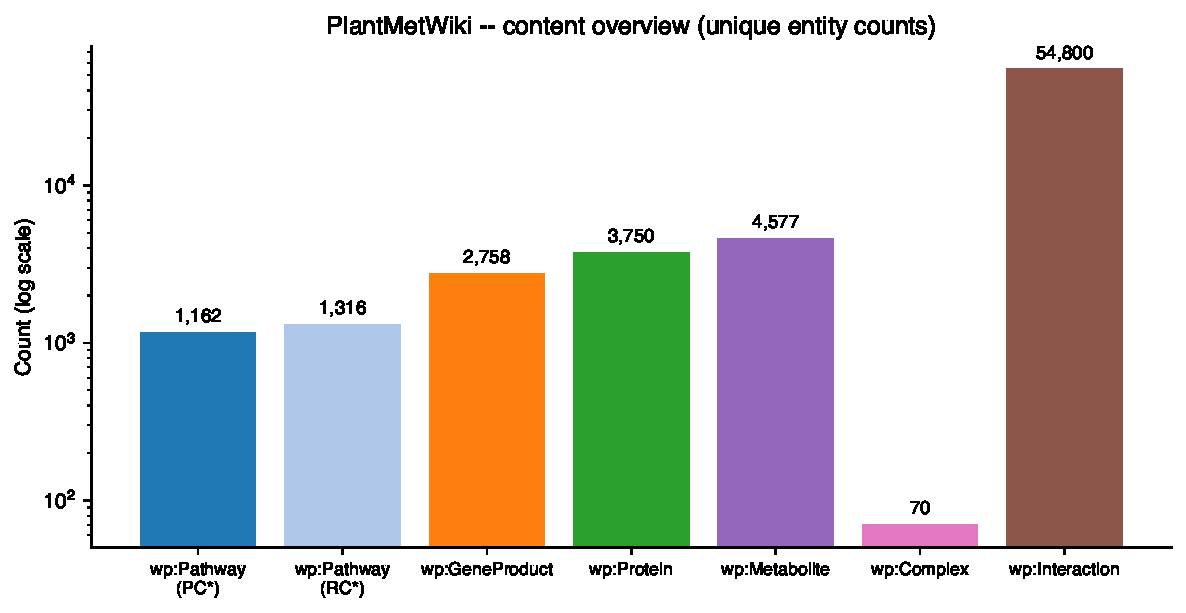
\includegraphics[width=0.86\textwidth]{supplementary_figures/figS1a.pdf}\\[1.2em]
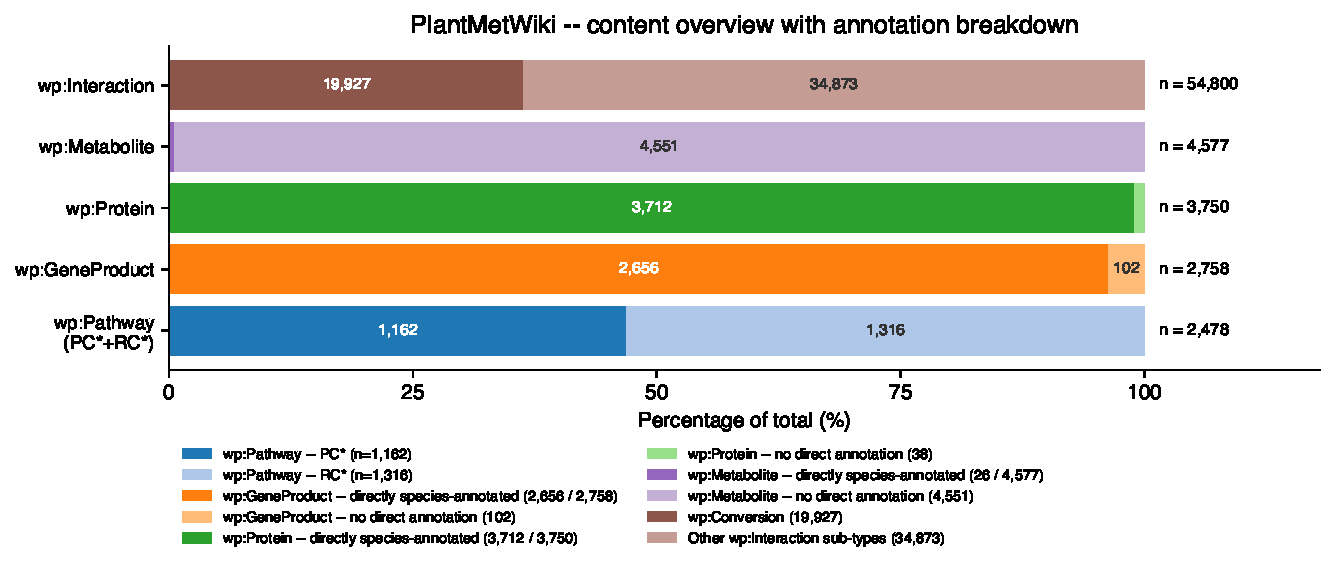
\includegraphics[width=\textwidth]{supplementary_figures/figS1b.pdf}
\end{center}

\captionof{figure}{\footnotesize \textbf{Top panel: Overview bar chart.} Total unique counts of the main
\texttt{wp:} content types in PlantMetWiki, on a logarithmic scale. Counts are true
\emph{distinct-entity} totals (\texttt{COUNT(DISTINCT ?e)} per class).
\texttt{wp:Pathway} (PC*) and \texttt{wp:Pathway} (RC*): pathways and reactions are both typed
\texttt{wp:Pathway} by the gpml2rdf converter and are distinguished only by their IRI prefix.
\texttt{wp:GeneProduct}, \texttt{wp:Protein}, \texttt{wp:Metabolite}, \texttt{wp:Complex}:
DataNode entity types from the WikiPathways vocabulary
(\url{http://vocabularies.wikipathways.org/wp#}). \texttt{wp:Interaction}: every instance of the
parent interaction class (covers all typed edges: \texttt{wp:Conversion}, \texttt{wp:Catalysis},
\texttt{wp:TranscriptionTranslation}, \texttt{wp:Inhibition}, \texttt{wp:Stimulation},
\texttt{wp:Binding}, \texttt{wp:ComplexBinding}).
\textbf{Bottom panel: PlantMetWiki core graph annotation coverage overview.} Proportional
breakdown (100\% per row) of each entity type by direct species-annotation status. Direct
annotation: the entity carries a \texttt{wp:organism} triple in
\texttt{graph/gpml-taxonomy-extra}, pointing to an NCBITaxon IRI
(\texttt{http://purl.obolibrary.org/obo/NCBITaxon\_*}). Dark colours: directly annotated; light
colours: no direct \texttt{wp:organism} triple. \textbf{Genes} (\texttt{wp:GeneProduct}):
2,656 / 2,758 annotated (96\%). \textbf{Enzymes} (\texttt{wp:Protein}): 3,712 / 3,750 annotated
(99\%). \textbf{Metabolites} (\texttt{wp:Metabolite}): only 26 / 4,577 carry a direct
\texttt{wp:organism}; the rest are species-neutral in the source PlantCyc data.
\textbf{Interactions}: split into \texttt{wp:Conversion} (biochemical reactions, brown) and all
other \texttt{wp:} sub-types (light brown).}
\label{figS:overview}

\clearpage

%------------------------------------------------------------------ S2
\begin{center}
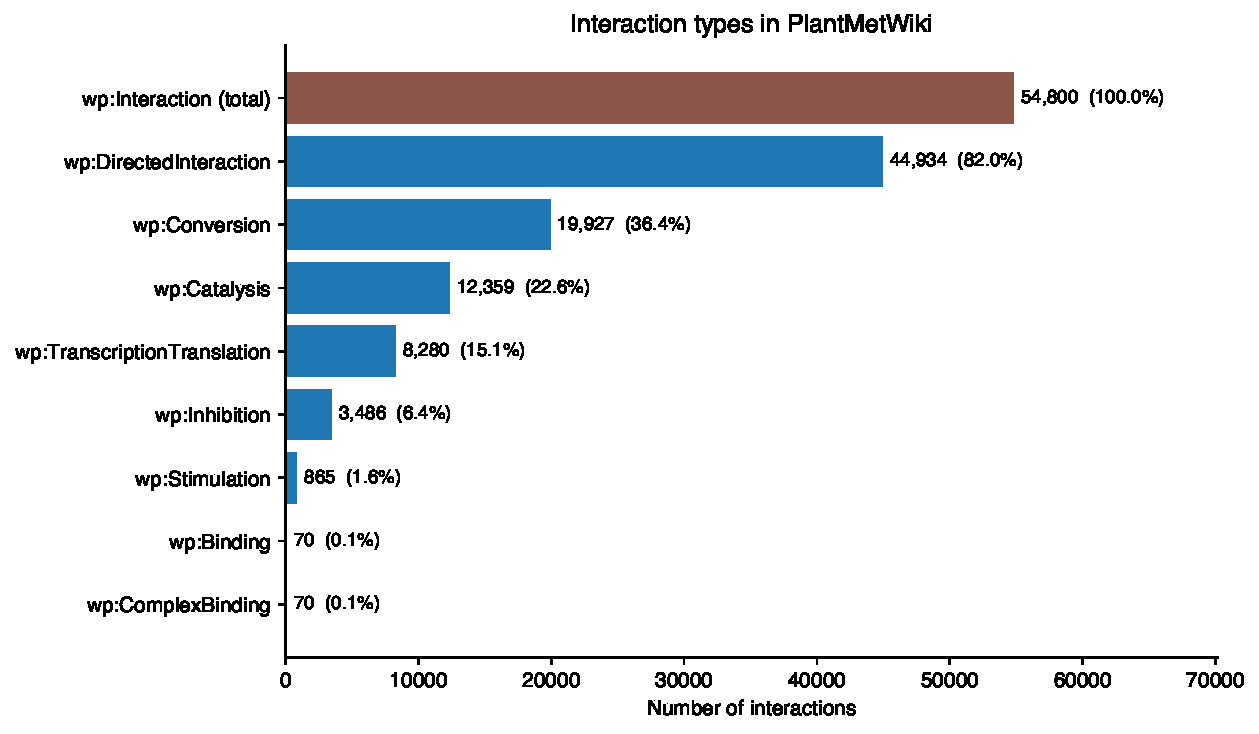
\includegraphics[width=\textwidth]{supplementary_figures/figS2.pdf}
\end{center}

\captionof{figure}{\footnotesize \textbf{Interaction type distribution.} \texttt{wp:Interaction} (parent
class) instances shown alongside each specific \texttt{wp:} interaction sub-type (WikiPathways
vocabulary, \url{http://vocabularies.wikipathways.org/wp#}). \texttt{wp:Conversion}: biochemical
transformation connecting a metabolite substrate to a metabolite product. \texttt{wp:Catalysis}:
link from an enzyme (\texttt{wp:GeneProduct} or \texttt{wp:Protein}) to the reaction it catalyses.
\texttt{wp:DirectedInteraction}: generic directed edge (used for transport, regulatory flow,
etc.). \texttt{wp:TranscriptionTranslation}: links gene, to transcript, to protein.
\texttt{wp:Inhibition}, \texttt{wp:Stimulation}: negative or positive regulatory effects.
\texttt{wp:Binding} or \texttt{wp:ComplexBinding}: physical interaction or complex formation.
Sub-type counts sum to more than the parent count because edges can carry multiple \texttt{wp:}
type labels.}
\label{figS:interactions}

\clearpage

%------------------------------------------------------------------ S3
\begin{center}
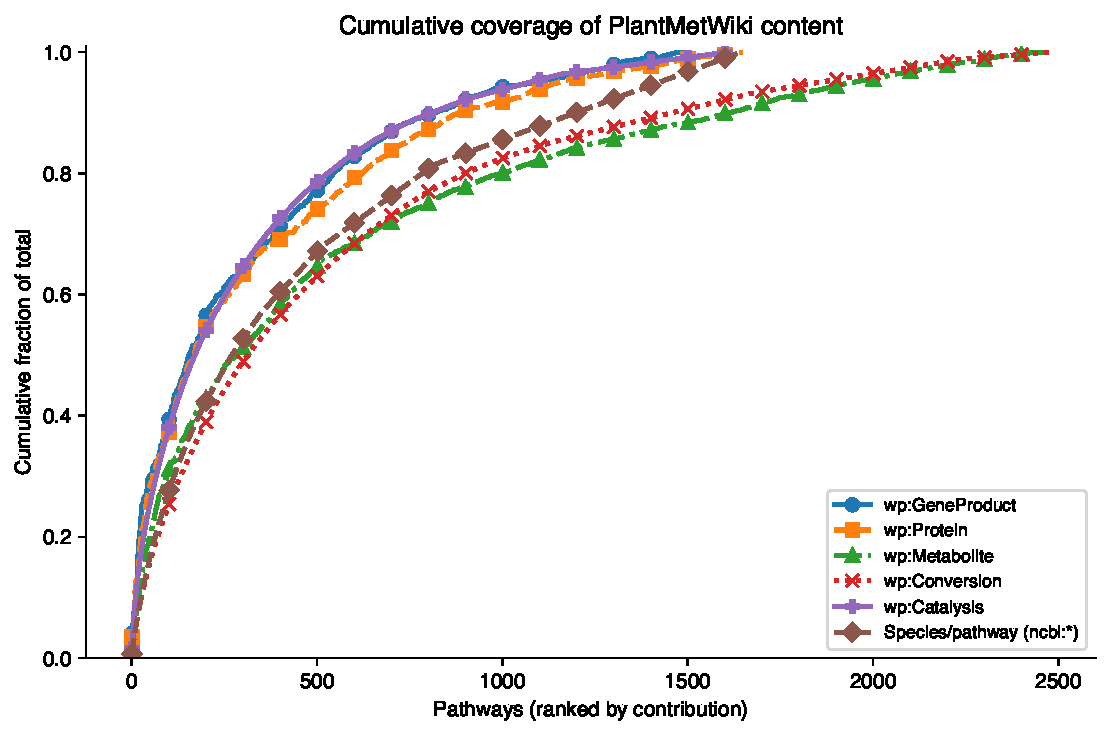
\includegraphics[width=\textwidth]{supplementary_figures/figS3.pdf}
\end{center}

\captionof{figure}{\footnotesize \textbf{PlantMetWiki core graph cumulative coverage curves.} For each
metric, pathways are ranked by count (highest first) and the cumulative fraction of the dataset
total is plotted against pathway rank. Pathway membership is encoded via
\texttt{dcterms:isPartOf}; entity types are \texttt{wp:GeneProduct}, \texttt{wp:Protein},
\texttt{wp:Metabolite}, and \texttt{wp:Conversion}. \texttt{wp:Conversion} and
\texttt{wp:Catalysis} interactions are minted with a pathway-specific IRI (each belongs to exactly
one pathway), so their per-pathway counts already sum exactly to the unique totals (19,927 and
12,359 respectively). \textbf{Species/pathway} is calculated differently from the other five
curves: for each pathway, \texttt{COUNT(DISTINCT ?taxon)} of species-specific
\texttt{wp:organism} annotations on any \texttt{wp:GeneProduct}/\texttt{wp:Protein} node
\texttt{dcterms:isPartOf} that pathway. A steep initial rise indicates concentration in a small
number of large pathways. Genes and enzymes rise steeply because \textit{Arabidopsis thaliana}
(NCBITaxon\_3702) pathways dominate the top ranks. The species-per-pathway curve rises more
slowly, reflecting that taxonomic diversity is distributed across many medium-sized pathways.
Curves that do not reach 100\% (metabolites reach $\sim$63\%, enzymes $\sim$95\%) indicate the
remaining unique entities have no recorded \texttt{dcterms:isPartOf} membership to any
\texttt{wp:Pathway}-typed resource in this ranking.}
\label{figS:cumulative}

\clearpage

%------------------------------------------------------------------ S4
\begin{center}
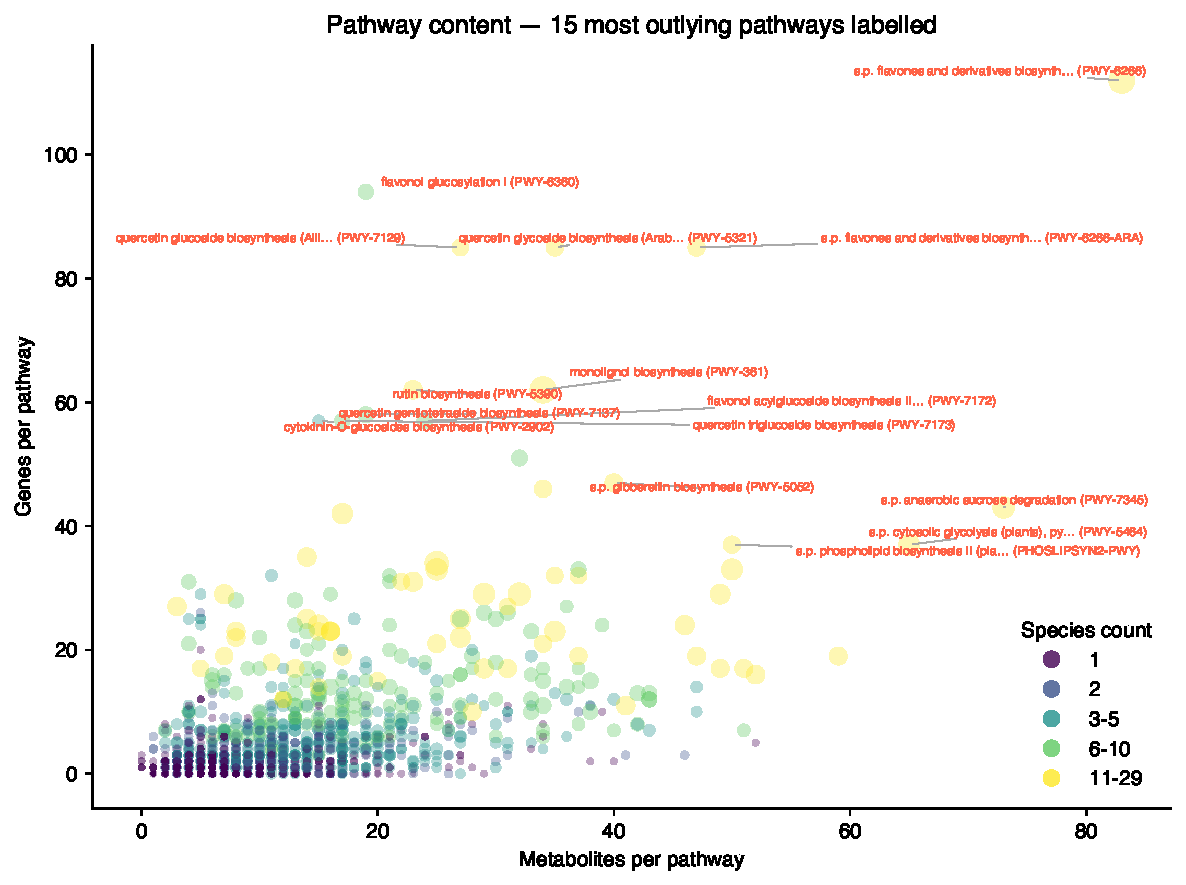
\includegraphics[width=\textwidth]{supplementary_figures/figS4.pdf}
\end{center}

\captionof{figure}{\footnotesize \textbf{PlantMetWiki core graph pathway content scatter plot with labelled
outliers.} Pathways plotted by metabolite and gene content, with point size encoding the number
of annotated species. Red rings and labels mark the 15 \texttt{wp:Pathway} objects furthest from
the point-cloud centroid (Euclidean distance in \texttt{wp:Metabolite} $\times$
\texttt{wp:GeneProduct} space). These outliers include large superpathways (aggregating many
sub-pathways via \texttt{dcterms:isPartOf}) and compound-rich maps where \texttt{wp:Metabolite}
nodes were imported without corresponding \texttt{wp:GeneProduct} annotations. Each label shows
the pathway title followed by its PlantCyc identifier in parentheses
(\texttt{dcterms:identifier} in \texttt{graph/gpml-properties-extra}, e.g. "PWY-6585", captured
from the GPML \texttt{<Property key="UniqueID">} during conversion: this is the code to look up
the same pathway directly in PlantCyc).}
\label{figS:scatter}

\clearpage

%------------------------------------------------------------------ S5
\begin{center}
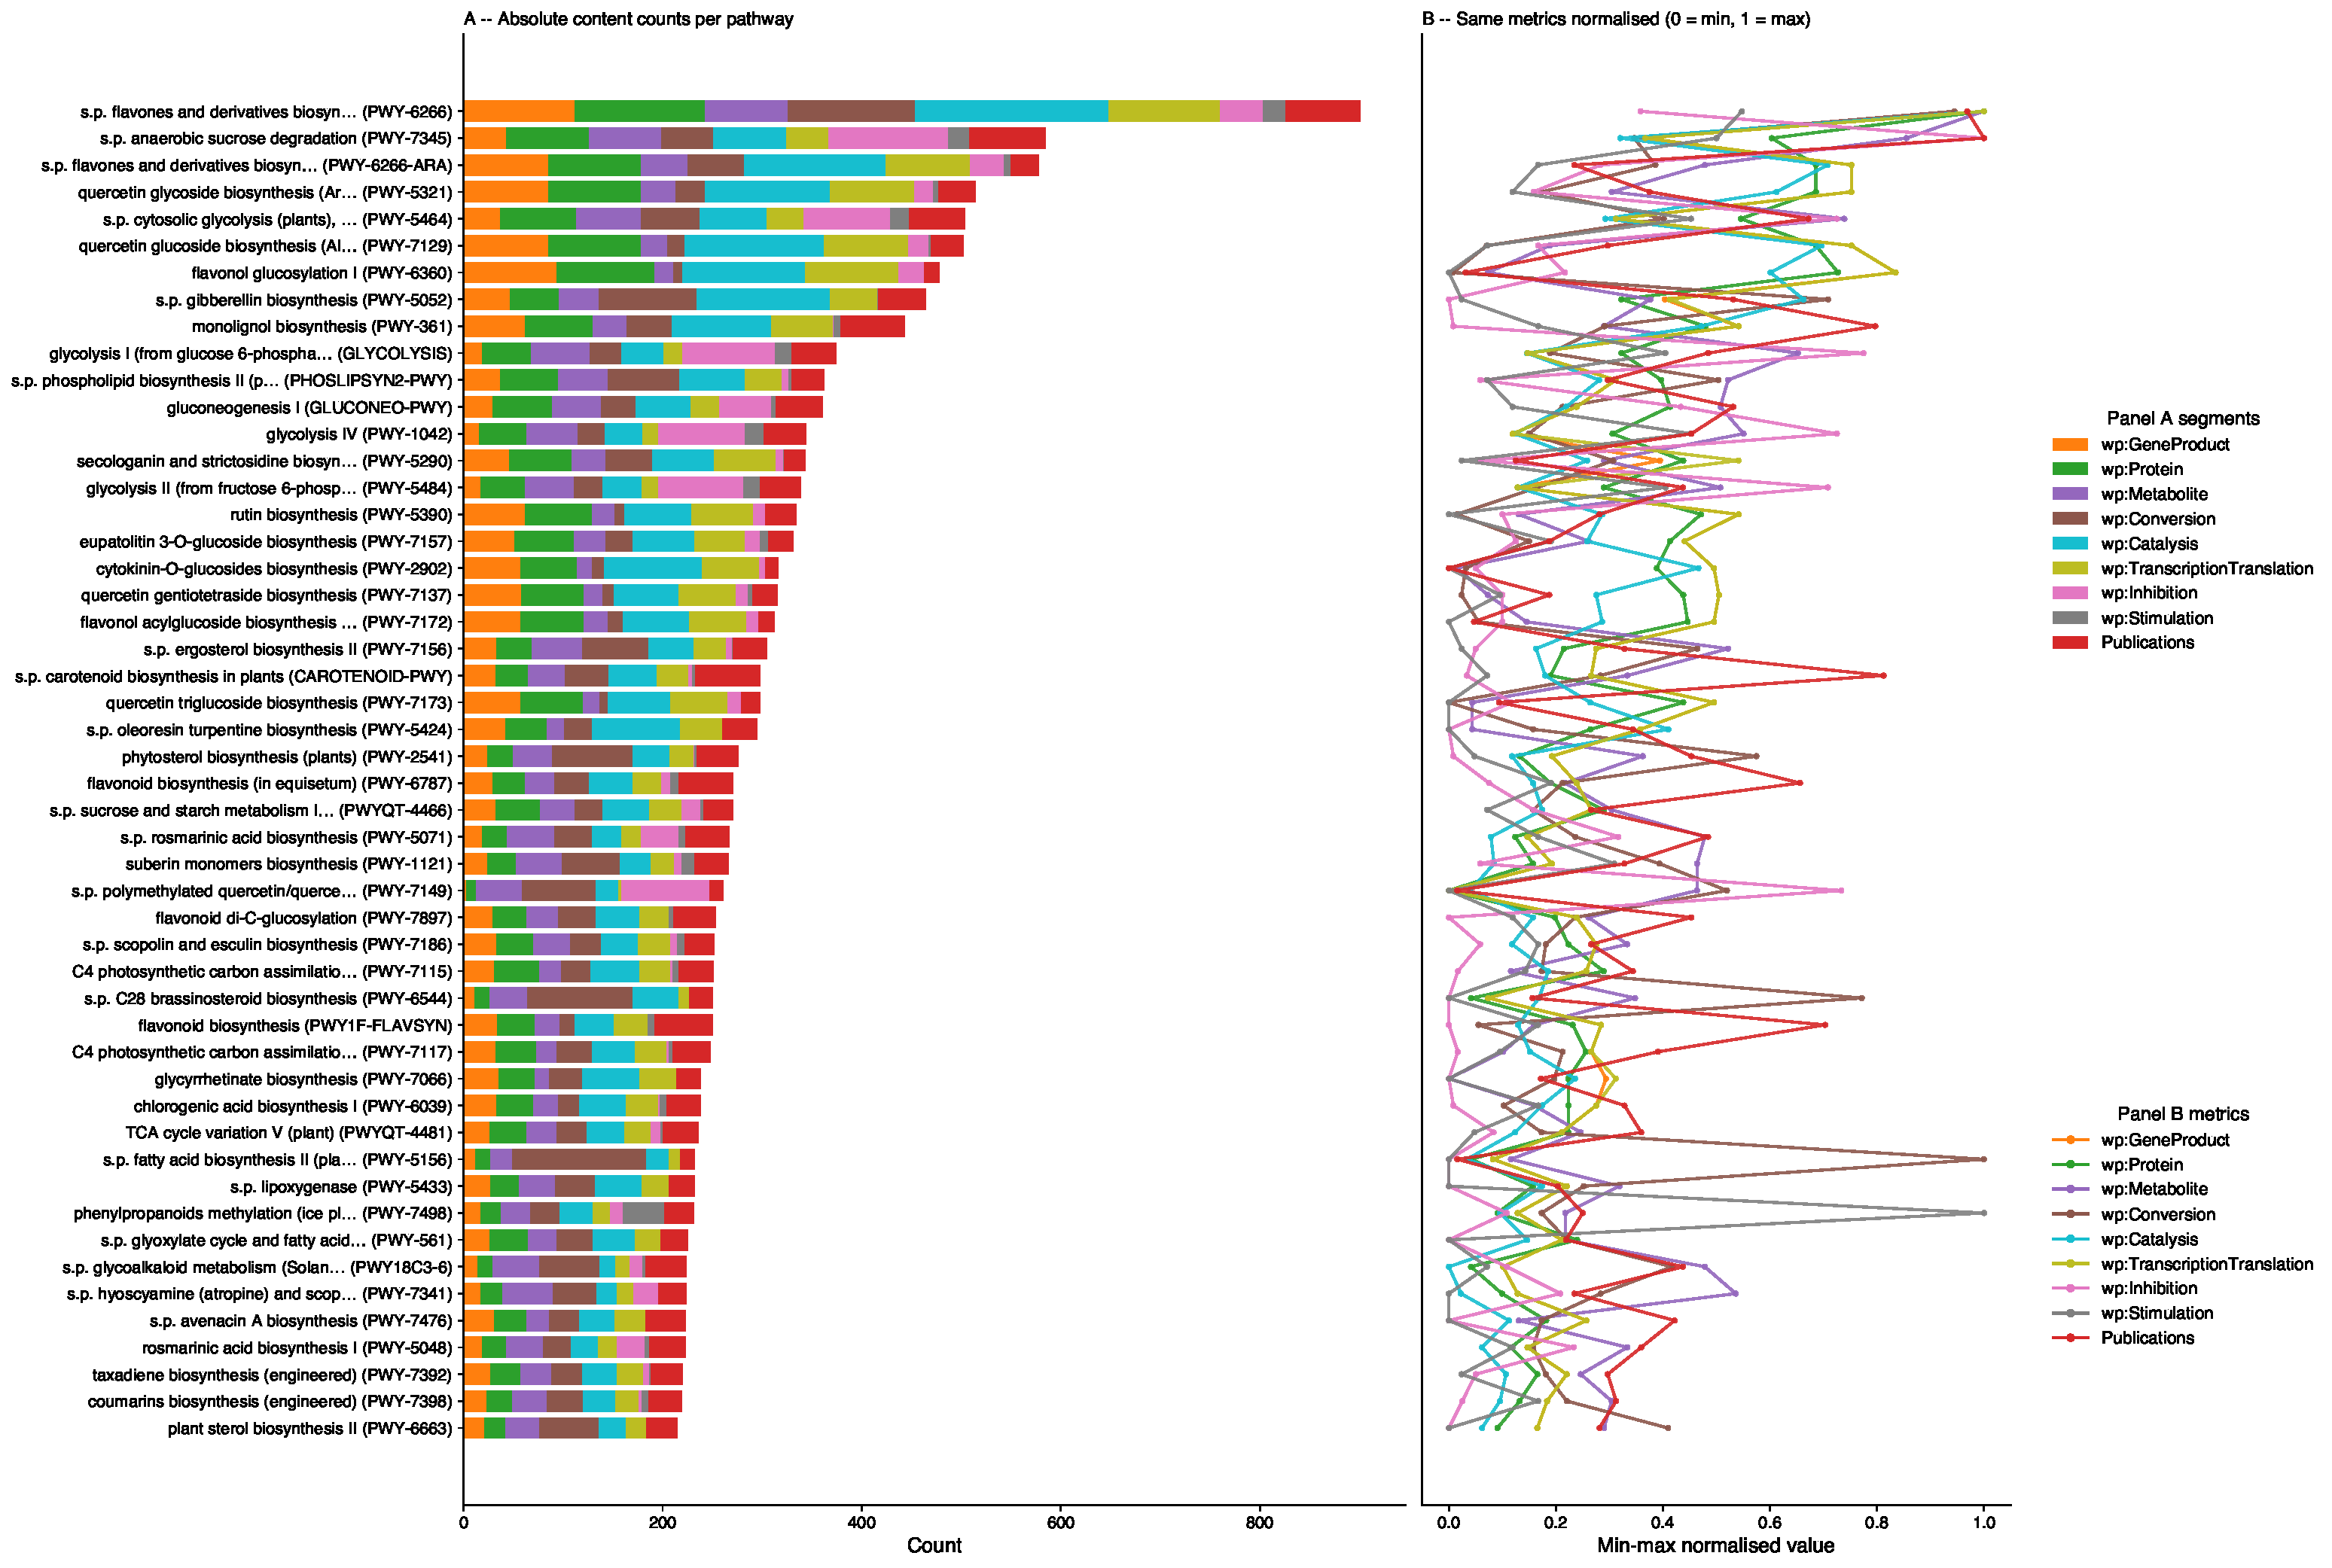
\includegraphics[width=\textwidth]{supplementary_figures/figS5.pdf}
\end{center}

\captionof{figure}{\footnotesize \textbf{Pathway content coverage (top 50 pathways).} Pathways ranked by
total content (sum of all nine metrics below), most content-rich at top. PlantCyc PWY/RXN
identifier shown in parentheses next to each pathway title (\texttt{dcterms:identifier} in
\texttt{graph/gpml-properties-extra}). \textbf{(A)} Absolute counts, horizontal stacked bars:
\texttt{wp:GeneProduct}, \texttt{wp:Protein}, \texttt{wp:Metabolite}, \texttt{wp:Conversion},
\texttt{wp:Catalysis}, \texttt{wp:TranscriptionTranslation}, \texttt{wp:Inhibition},
\texttt{wp:Stimulation} (all \texttt{dcterms:isPartOf} that pathway), and linked publications
(\texttt{dcterms:references}/\texttt{cito:cites} on the pathway itself). \textbf{(B)} Min--max
normalization (0 = minimum, 1 = maximum across the top 50 pathways) of the same nine metrics.
Unlike the species figure, there is no direct/indirect distinction here: every count is already
scoped to a single pathway via direct RDF membership, so no catalysis-chain tracing is needed.}
\label{figS:pathwaycoverage}

\clearpage

%------------------------------------------------------------------ S6
\begin{center}
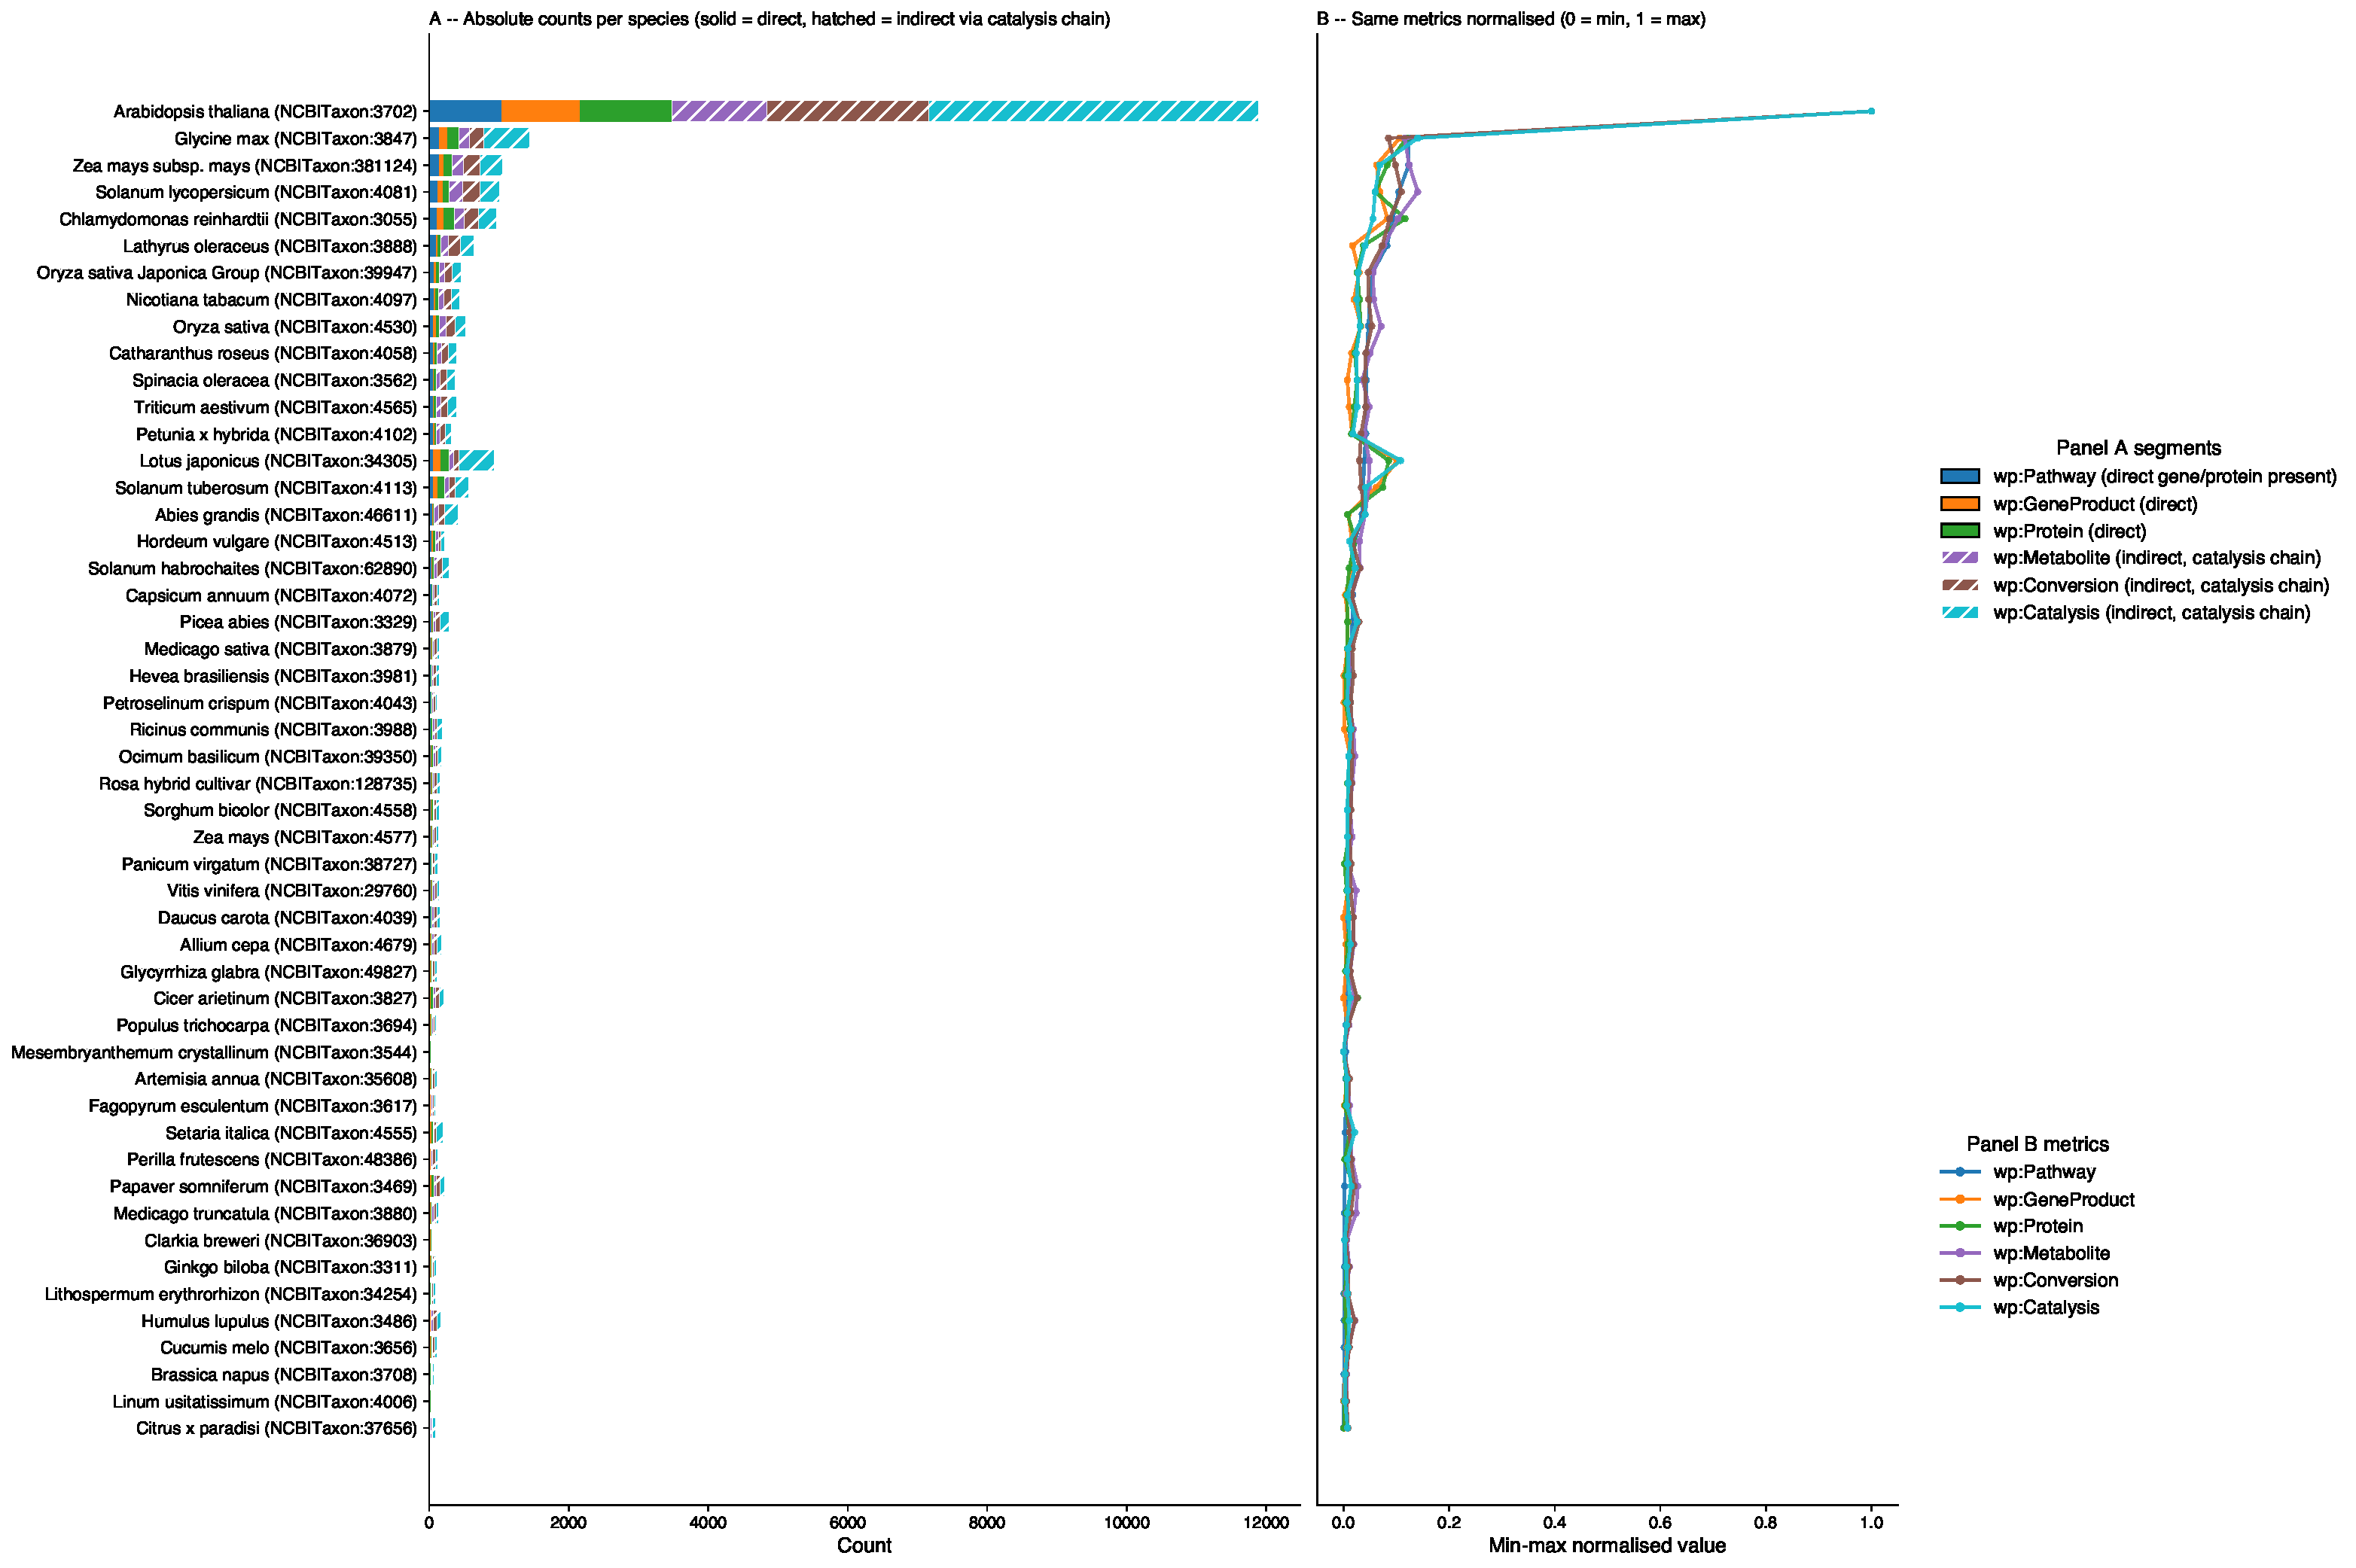
\includegraphics[width=\textwidth]{supplementary_figures/figS6.pdf}
\end{center}

\captionof{figure}{\footnotesize \textbf{PlantMetWiki core graph species coverage (top 50 species).} Both
panels share the same vertical species axis (most pathway-rich at top), avoiding rotated category
labels. \textbf{(A)} Absolute counts, horizontal stacked bars. Solid: \texttt{wp:Pathway}
(containing a direct gene/protein of the species), \texttt{wp:GeneProduct}/\texttt{wp:Protein}
with a direct \texttt{wp:organism} annotation. Hatched: \texttt{wp:Metabolite},
\texttt{wp:Conversion}, and \texttt{wp:Catalysis} attributed indirectly via the specific catalysis
chain (\texttt{wp:source}/\texttt{wp:target}) the species' enzyme participates in (not broad
pathway co-occurrence). Publications are not included (pathway-level only, not
chain-attributable). \textbf{(B)} Min--max normalisation (0 = minimum, 1 = maximum across the top
50 species) of: pathways, genes (\texttt{wp:GeneProduct}), enzymes (\texttt{wp:Protein}),
metabolites (\texttt{wp:Metabolite}), conversions (\texttt{wp:Conversion}), and catalysis
(\texttt{wp:Catalysis}). Normalisation reveals cross-species patterns independent of the large
absolute differences driven by \textit{Arabidopsis thaliana} (NCBITaxon\_3702).}
\label{figS:speciescoverage}

\clearpage

%------------------------------------------------------------------ S7
\begin{center}
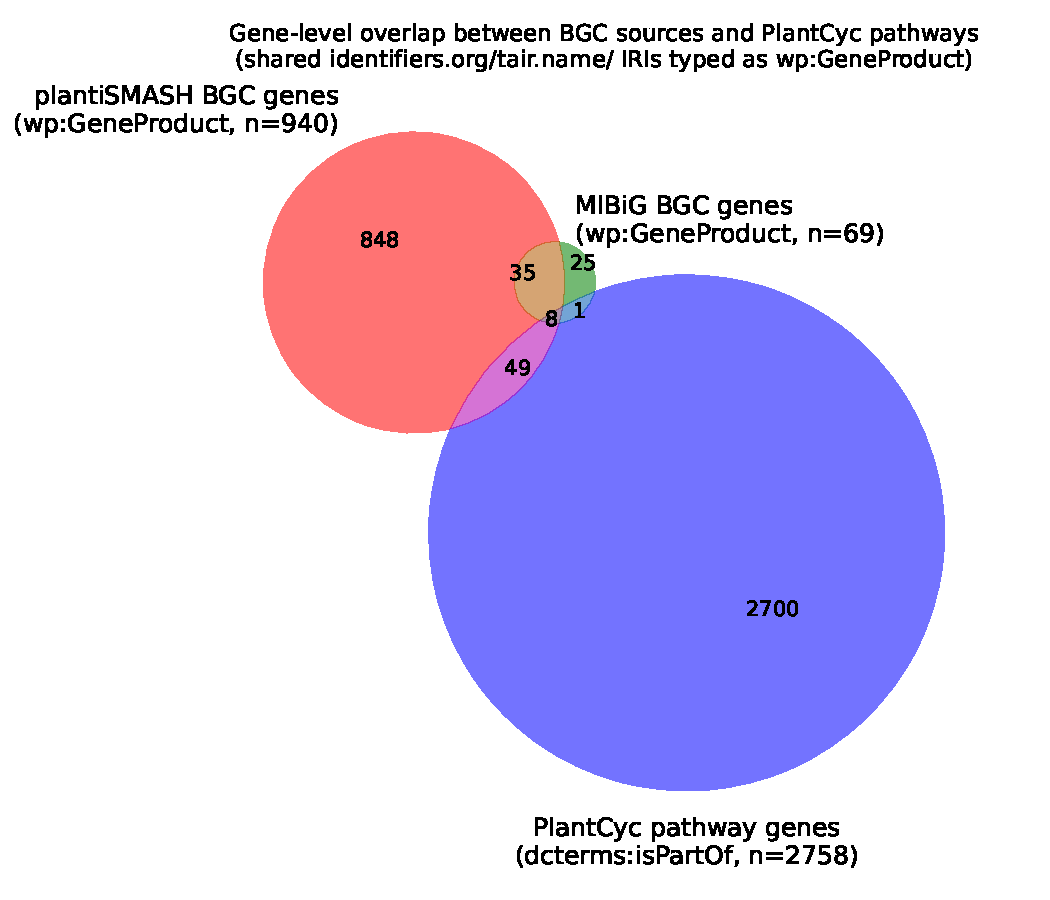
\includegraphics[width=0.92\textwidth]{supplementary_figures/figS7.pdf}
\end{center}

\captionof{figure}{\footnotesize \textbf{Gene-level overlap between Biosynthetic Gene Cluster (BGC) sources
and PlantCyc pathway annotations in PlantMetWiki.} Sets represent all \texttt{wp:GeneProduct}
gene members identified by \texttt{identifiers.org/tair.name/} IRIs: plantiSMASH BGC genes
($n = 940$), MIBiG BGC genes ($n = 69$), and PlantCyc pathway genes ($n = 2{,}758$; all genes with
\texttt{dcterms:isPartOf} a \texttt{wp:Pathway} in \texttt{graph/pathways}). Only
\texttt{wp:GeneProduct} nodes (with identifiers.org IRIs) can form cross-graph joins;
\texttt{pmw:MemberIdentifier} nodes (403 in MIBiG, 0 in plantiSMASH) are excluded. Of the 940
plantiSMASH BGC genes, 57 (6\%) overlap with at least one PlantCyc pathway gene; for MIBiG, 9 of
69 (13\%). 35 genes are shared between the plantiSMASH and MIBiG BGC graphs but absent from any
current PlantCyc pathway.}
\label{figS:bgcvenn}

\clearpage

%------------------------------------------------------------------ S8
\begin{center}
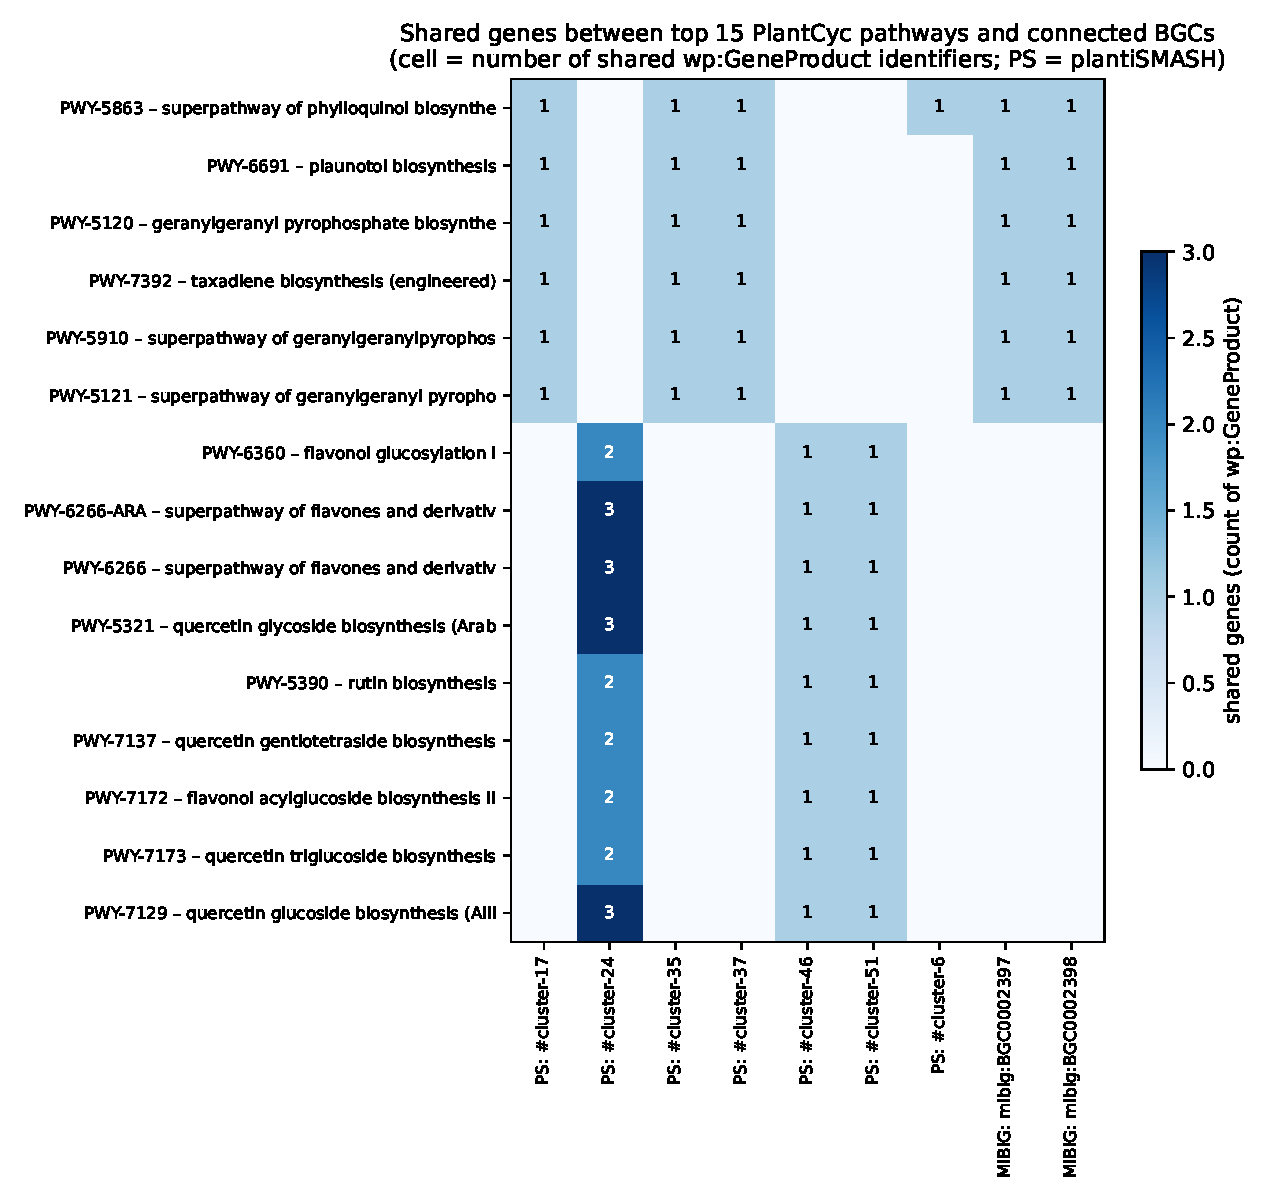
\includegraphics[width=0.95\textwidth]{supplementary_figures/figS8.pdf}
\end{center}

\captionof{figure}{\footnotesize \textbf{MIBiG to plantiSMASH BGC coverage representation.} Gene-sharing
matrix between the top 15 PlantCyc pathways (ranked by number of connected BGCs) and individual
Biosynthetic Gene Clusters from plantiSMASH (PS:) and MIBiG. Rows are PlantCyc pathways labelled
by their stable accession (PWY/RXN ID from \texttt{graph/gpml-properties-extra}) and title
(truncated to 38 characters). Columns are individual BGC labels. Cell values show the count of
shared \texttt{wp:GeneProduct} IRIs (\texttt{identifiers.org/tair.name/}) between a pathway and a
BGC; empty cells indicate no shared gene. Full crosslink data (all 225 BGC--gene--pathway
triples) is in Supplementary Table S5.}
\label{figS:bgcmatrix}

\clearpage

%------------------------------------------------------------------ S9
\begin{center}
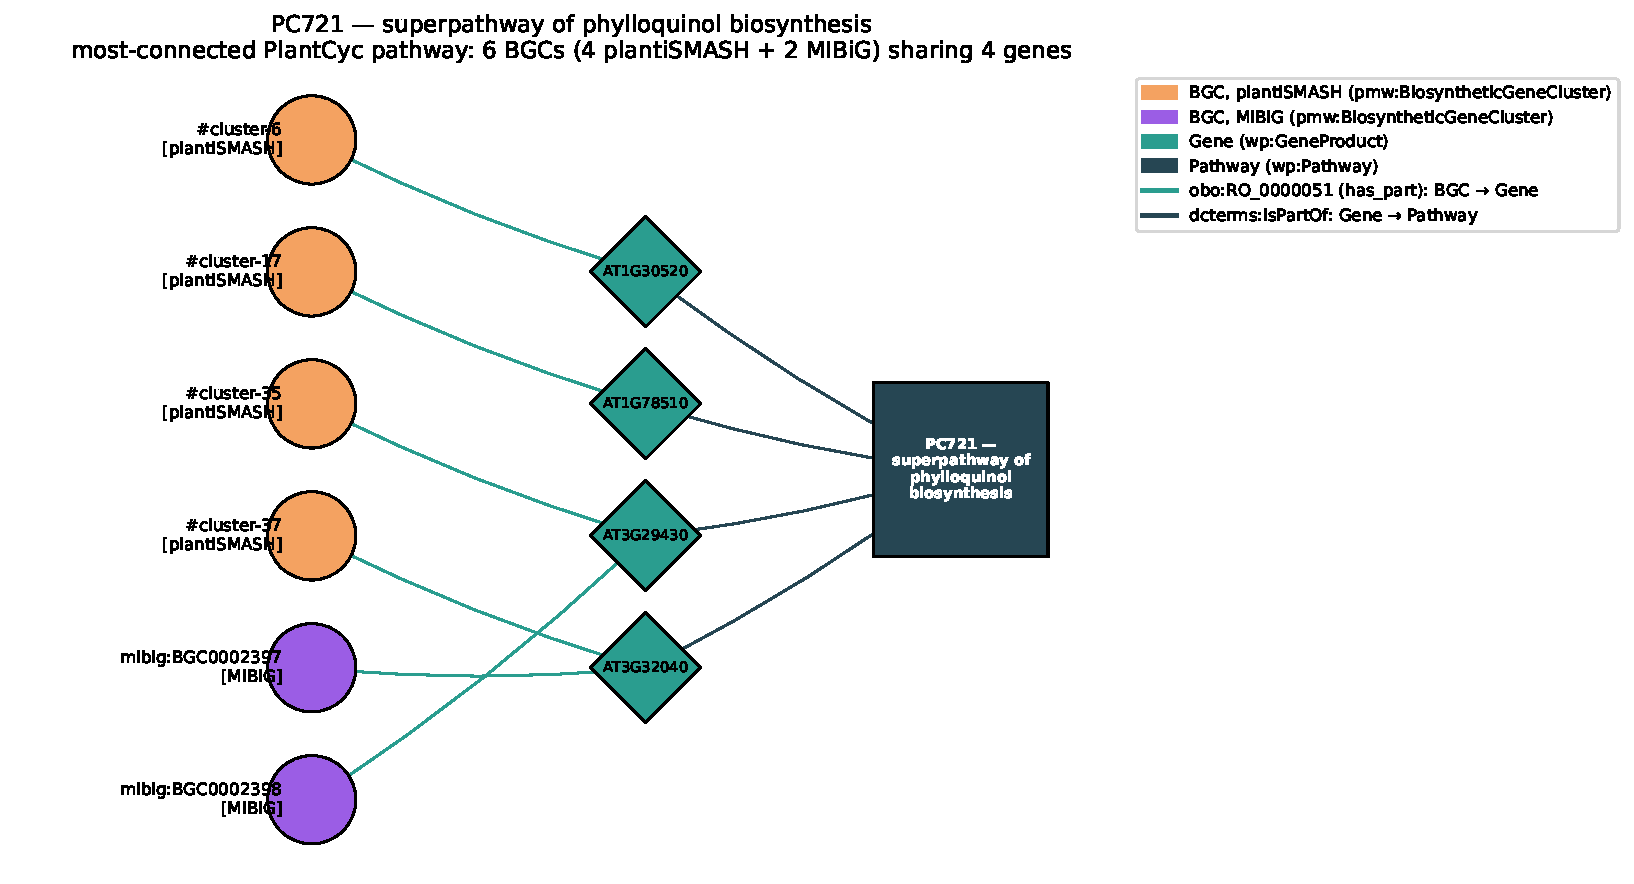
\includegraphics[width=\textwidth]{supplementary_figures/figS9.pdf}
\end{center}

\captionof{figure}{\footnotesize \textbf{RDF network of the most-connected PlantCyc pathway} (PC721 /
PWY-5863, \textit{superpathway of phylloquinol biosynthesis}), showing all Biosynthetic Gene
Clusters linked to it via shared \texttt{wp:GeneProduct} gene members. Circles (left) represent
BGCs (\texttt{pmw:BiosyntheticGeneCluster}), coloured by source: plantiSMASH (orange, $n = 4$) and
MIBiG (purple, $n = 2$). Diamonds (centre) represent shared genes (\texttt{wp:GeneProduct},
$n = 4$), labelled by their TAIR locus identifier. The square (right) represents the PlantCyc
pathway (\texttt{wp:Pathway}). Green edges: \texttt{obo:RO\_0000051} (\texttt{has\_part}, BGC to
gene edge); dark edges: \texttt{dcterms:isPartOf} (gene to pathway edge). This tripartite layout
illustrates the SPARQL join mechanism between \texttt{graph/bgc-*} and \texttt{graph/pathways} via
the shared identifiers.org IRI space: a gene appearing in both a BGC graph and the pathway graph
provides the cross-graph link without requiring any pre-computed mapping table.}
\label{figS:bgcnetwork}

\clearpage

%------------------------------------------------------------------ S10
\begin{center}
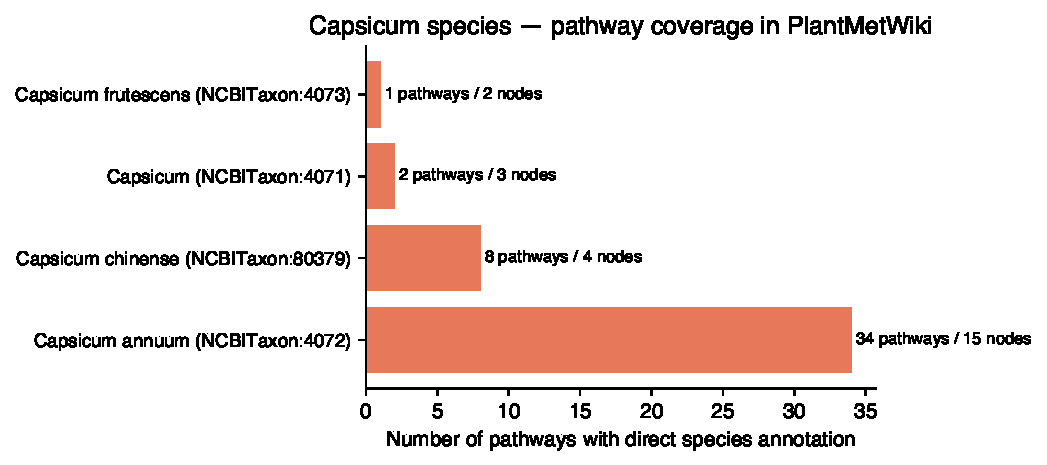
\includegraphics[width=0.80\textwidth]{supplementary_figures/figS10a.pdf}\\[1.2em]
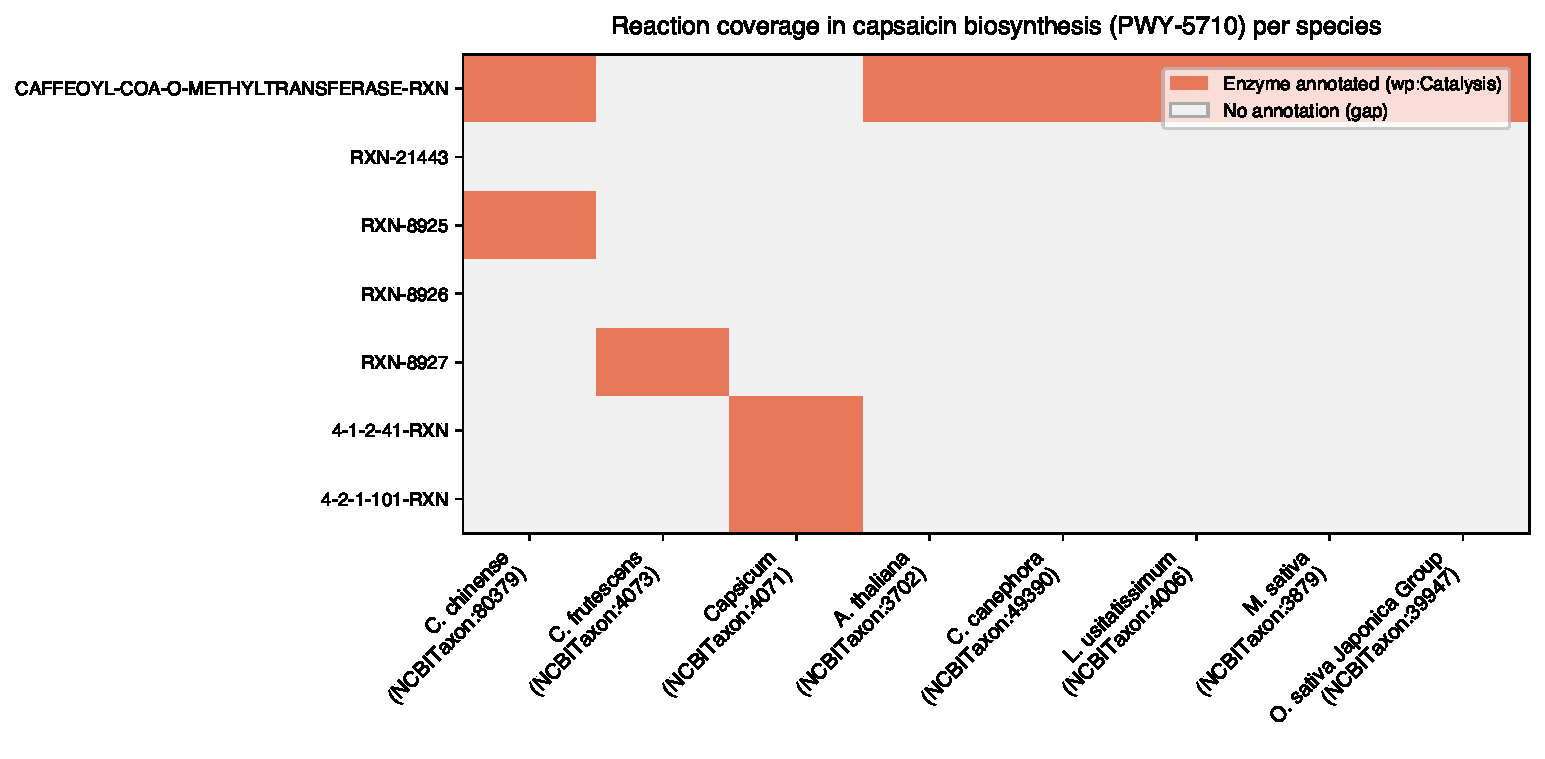
\includegraphics[width=\textwidth]{supplementary_figures/figS10b.pdf}
\end{center}

\captionof{figure}{\footnotesize \textbf{Top panel: Pathway coverage of \textit{Capsicum} species in
PlantMetWiki.} Bars show the number of pathways for which each taxon has at least one directly
annotated \texttt{wp:GeneProduct} or \texttt{wp:Protein} DataNode (\texttt{wp:organism} in
\texttt{graph/gpml-taxonomy-extra}). The annotation count (number of annotated nodes and pathways)
is shown beside each bar. \textit{Capsicum annuum} (NCBITaxon:4072) is the most extensively
curated \textit{Capsicum} entry in PlantCyc (CapsicumCyc), covering 34 pathways, while
\textit{C. chinense} (NCBITaxon:80379), \textit{C. frutescens} (NCBITaxon:4073), and the genus
\textit{Capsicum} (NCBITaxon:4071) have substantially lower annotation depth.
\textbf{Bottom panel: Reaction coverage matrix for capsaicin biosynthesis} (PWY-5710) across all
annotated species. Rows are \texttt{wp:Conversion} reactions (PlantCyc reaction accession IDs);
columns are species with at least one annotated enzyme in this pathway, labelled with abbreviated
binomial name and NCBITaxon identifier. Orange = at least one \texttt{wp:Protein} or
\texttt{wp:GeneProduct} DataNode linked via \texttt{wp:Catalysis}; grey = annotation gap.
\textit{Capsicum annuum} (NCBITaxon:4072) is absent from this matrix --- it has no directly
annotated enzyme in this pathway despite being the most pathway-rich \textit{Capsicum} species in
PlantMetWiki overall (34 pathways). Cross-species inference candidates are reactions covered in
\textit{C. chinense}, \textit{C. frutescens}, or the genus \textit{Capsicum}.}
\label{figS:capsicum}

\clearpage

%------------------------------------------------------------------ S11
\begin{center}
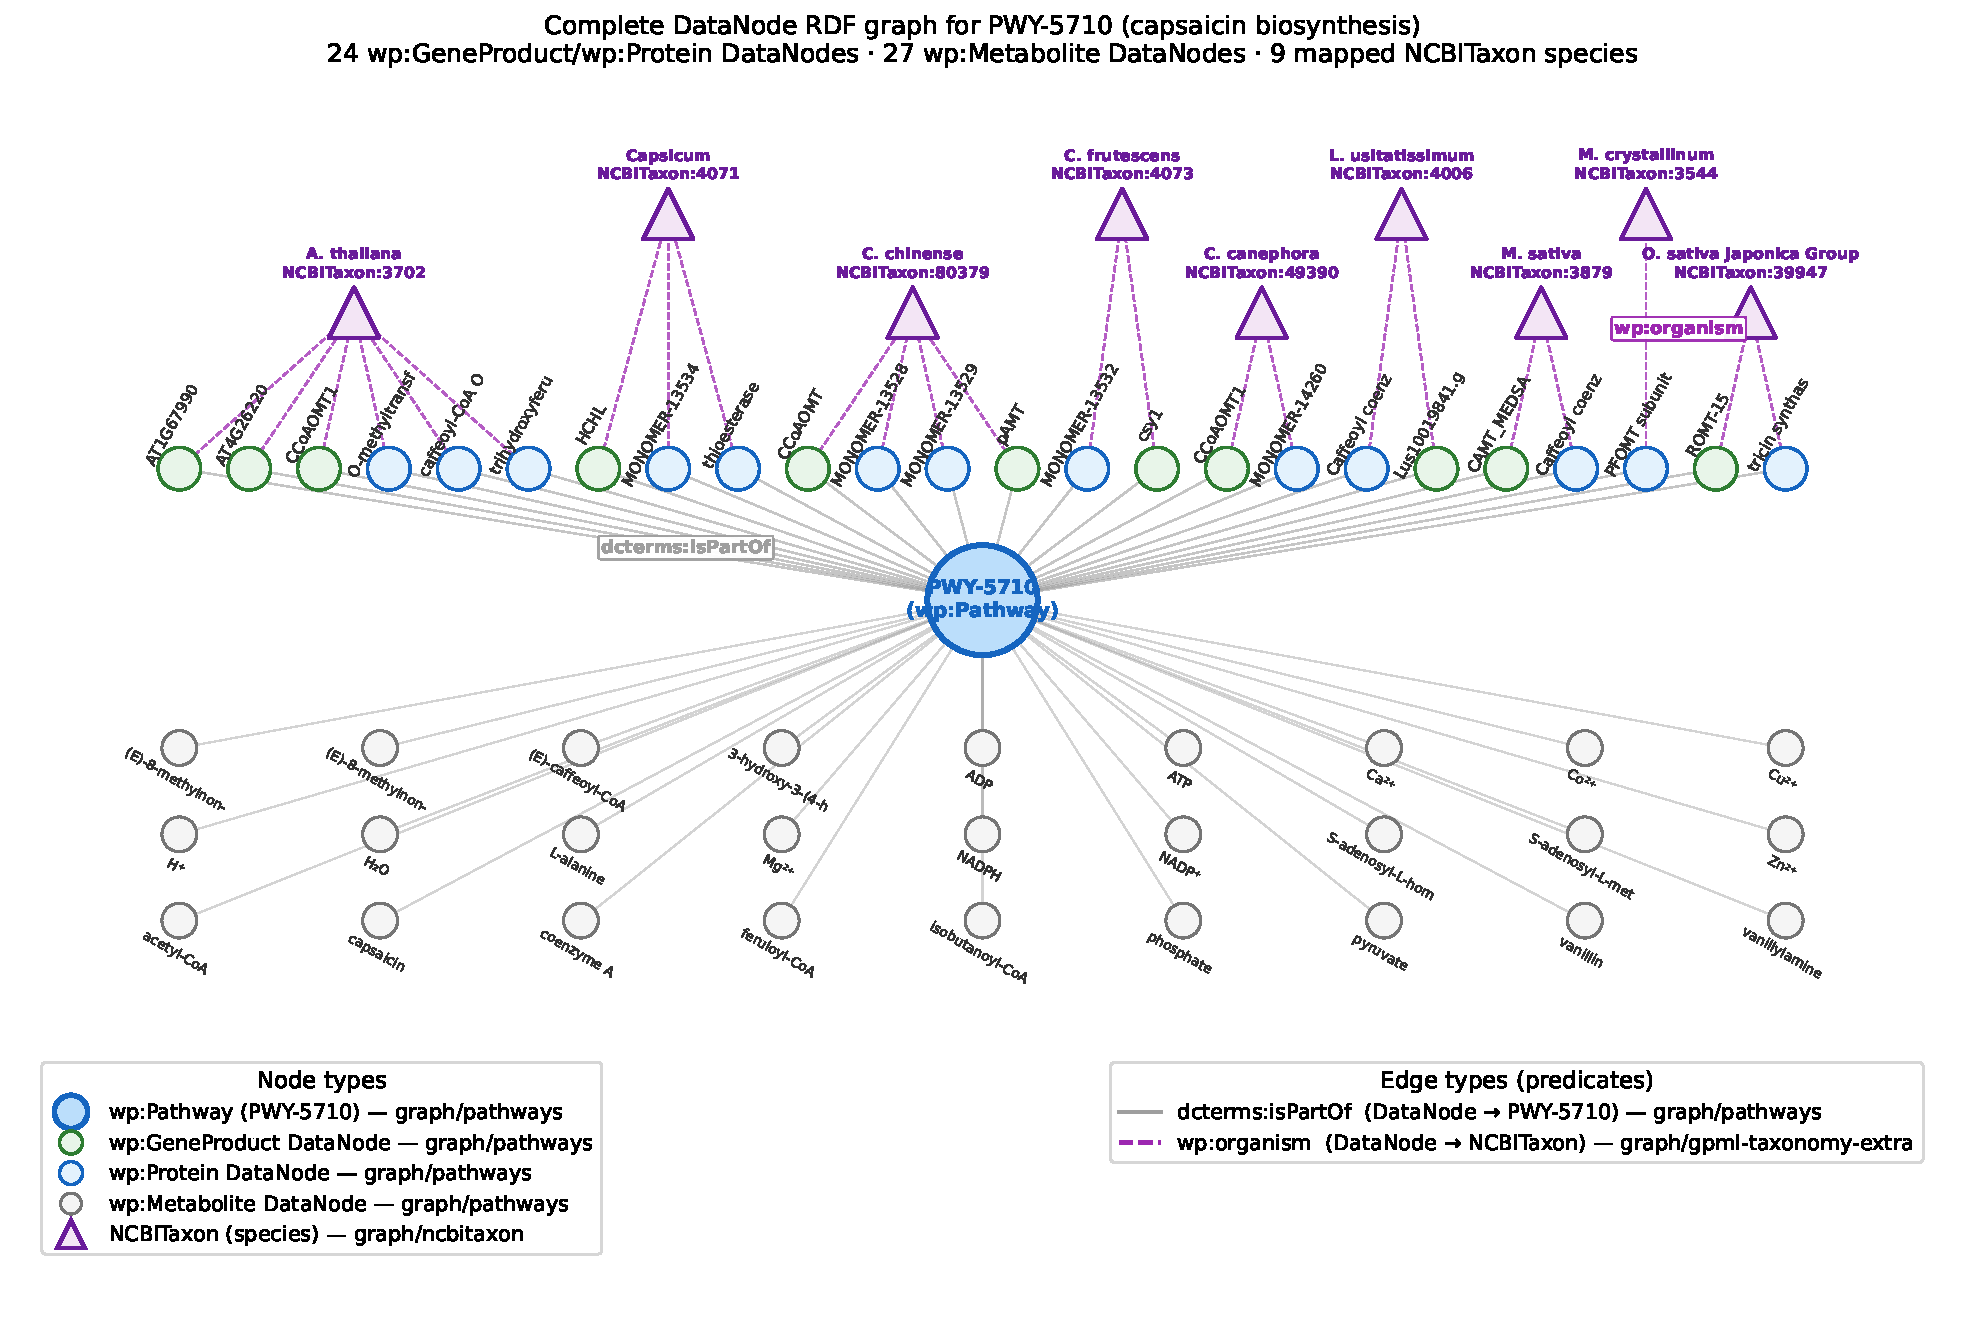
\includegraphics[width=\textwidth]{supplementary_figures/figS11.pdf}
\end{center}

\captionof{figure}{\footnotesize \textbf{All DataNodes in capsaicin biosynthesis (PWY-5710) and their
species annotations across the two RDF graphs.} The
\texttt{wp:GeneProduct}/\texttt{wp:Protein} DataNodes (green/blue circles) are arranged in a
horizontal row, sorted by associated species, and connect to PWY-5710 (centre,
\texttt{wp:Pathway}) via \texttt{dcterms:isPartOf} (solid grey edges, \texttt{graph/pathways}).
Labels show the DataNode name (up to 14 characters, rotated). The \texttt{wp:Metabolite}
DataNodes (grey circles, below) connect the same way: 27 \texttt{wp:Metabolite} nodes carry no
direct species annotation and are shared across all annotated species. NCBITaxon species nodes
(purple triangles, above) are labelled with abbreviated binomial name and NCBITaxon accession,
connected to their annotated DataNodes via \texttt{wp:organism} (dashed purple edges,
\texttt{graph/gpml-taxonomy-extra}). One representative edge label per predicate type is shown
for clarity.}
\label{figS:capsaicinnodes}

\clearpage

%------------------------------------------------------------------ S12
\begin{center}
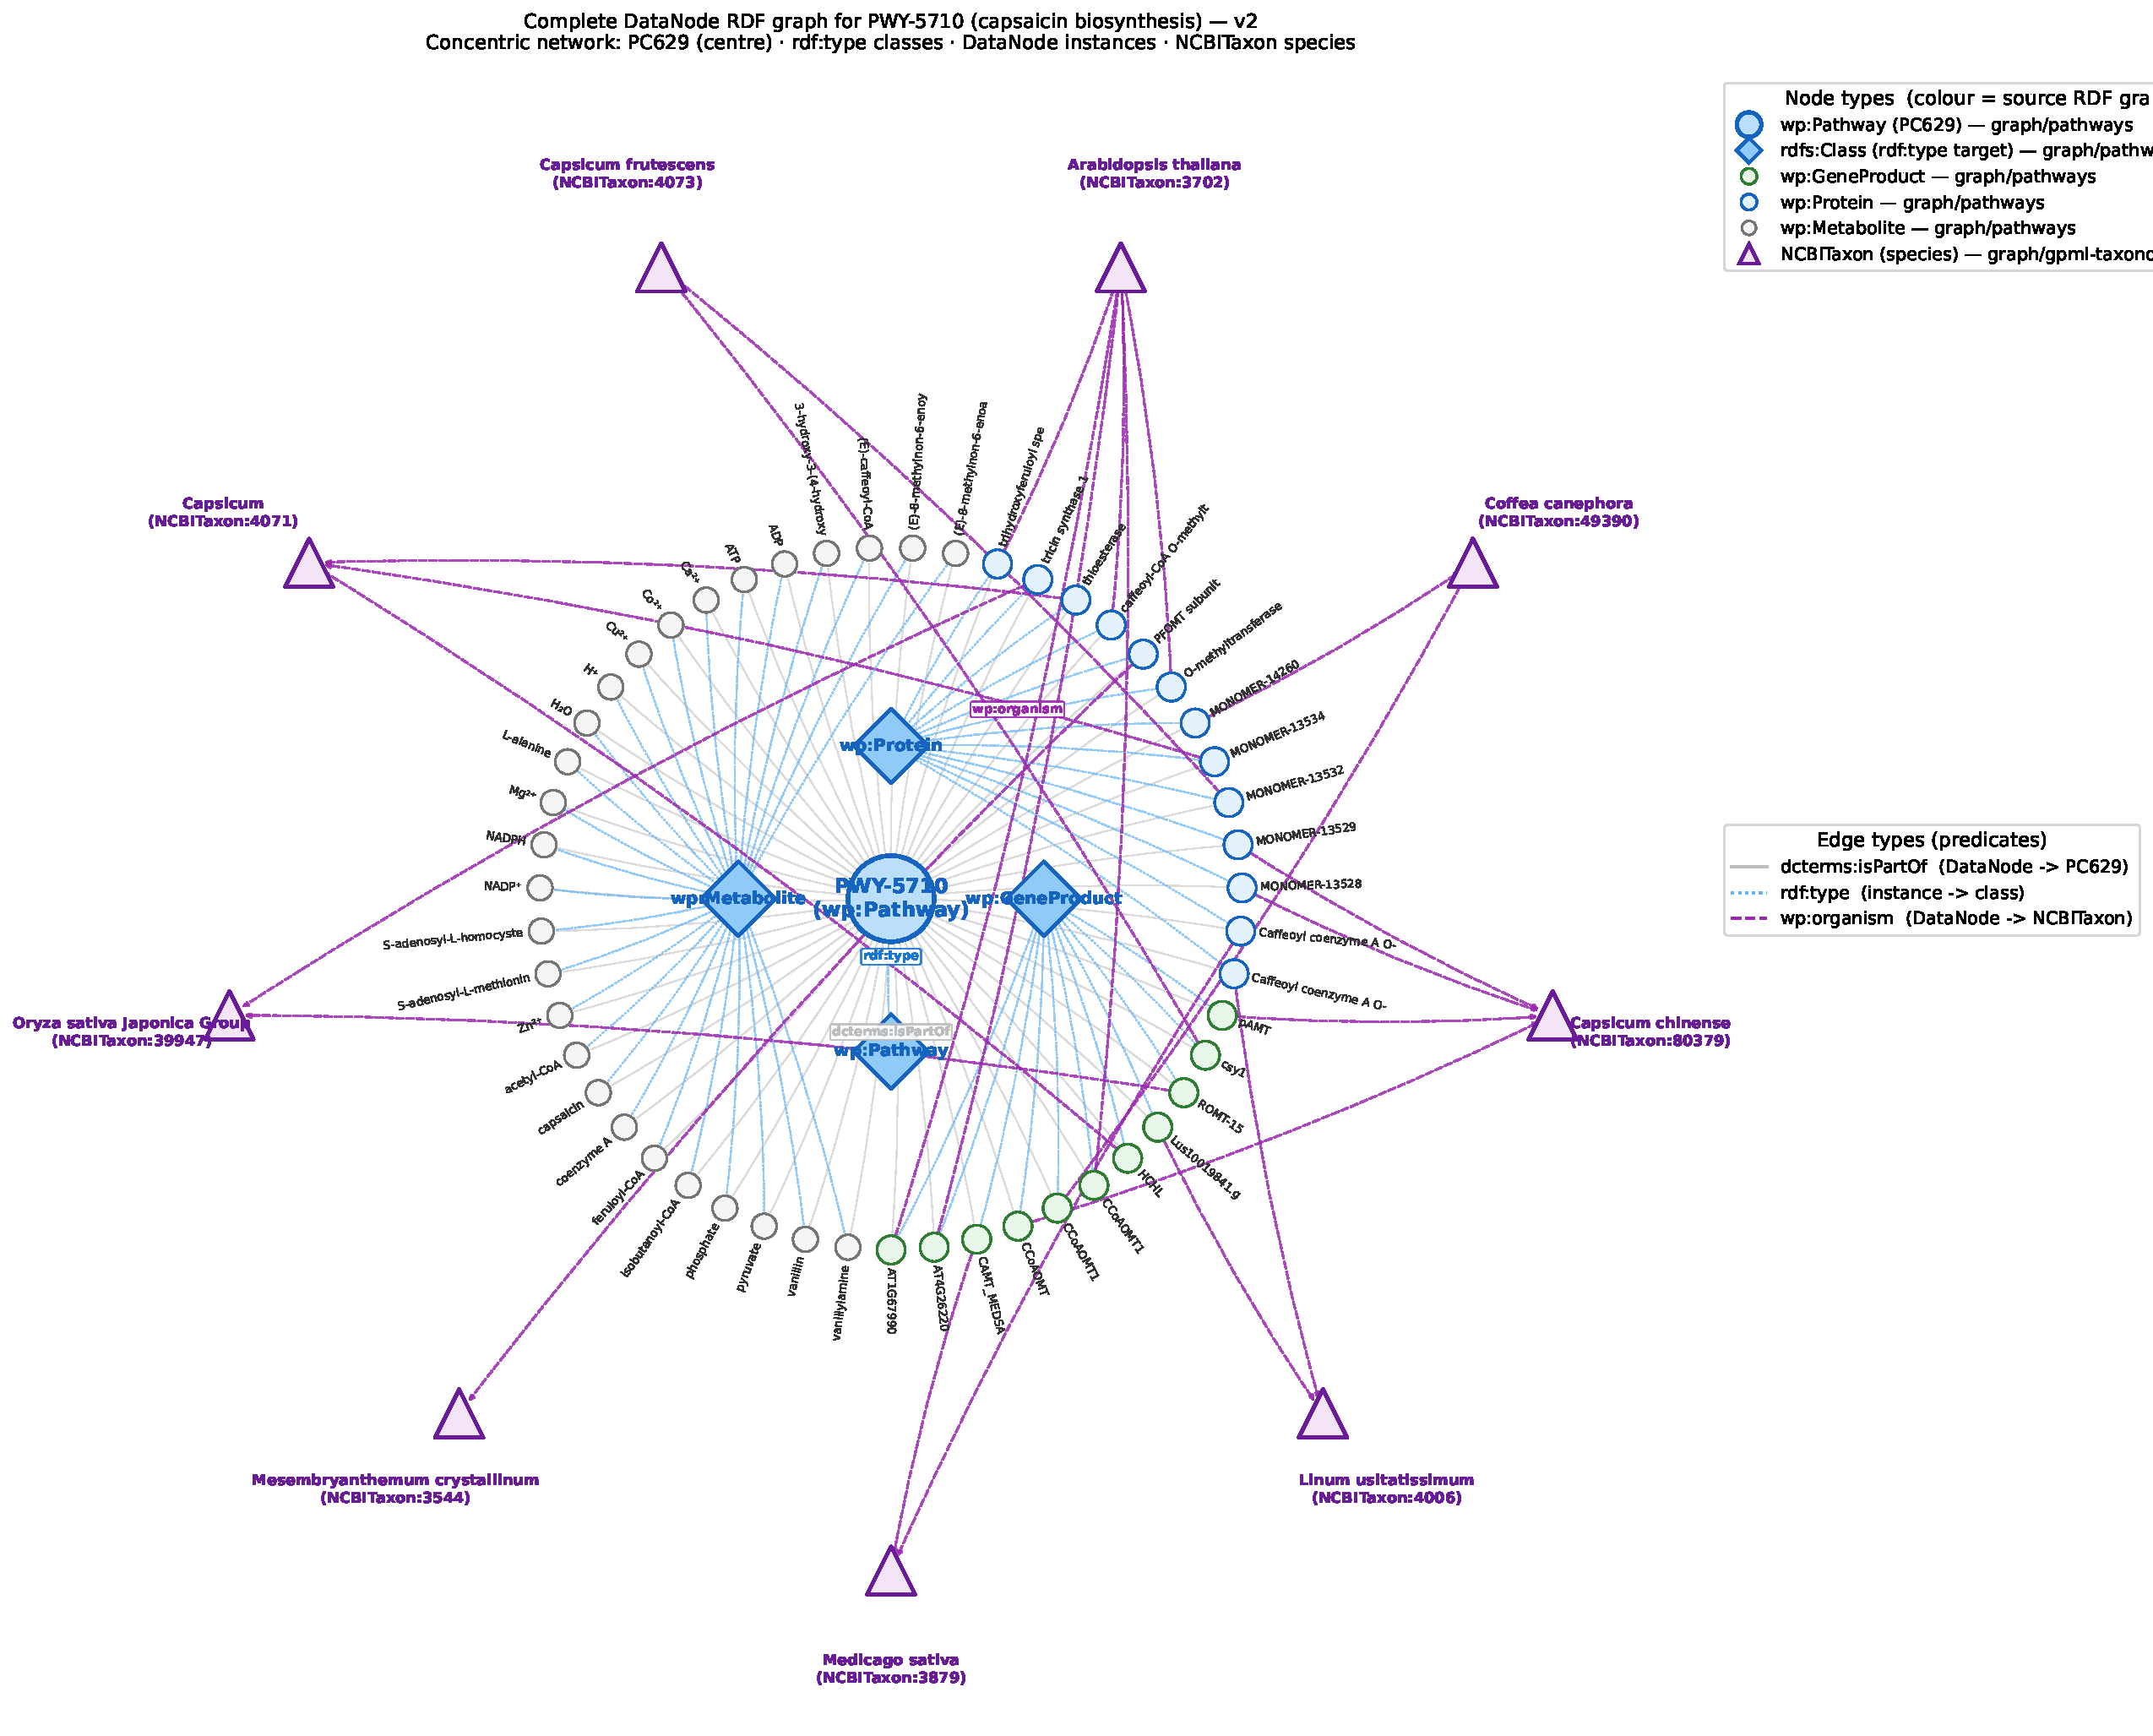
\includegraphics[width=\textwidth]{supplementary_figures/figS12.pdf}
\end{center}

\captionof{figure}{\footnotesize \textbf{Complete DataNode RDF graph for capsaicin biosynthesis (PWY-5710)
concentric network.} Every node is an individual RDF resource and every edge an individual triple.
PWY-5710 (\texttt{wp:Pathway}, large blue circle) sits at the centre; ring 1 holds the four
\texttt{rdfs:Class} nodes reachable via \texttt{rdf:type}; ring 2 holds all 51 DataNode instances
(11 \texttt{wp:GeneProduct}, 13 \texttt{wp:Protein}, 27 \texttt{wp:Metabolite}), each linked to
PWY-5710 via \texttt{dcterms:isPartOf} (grey solid edges) and to its class via \texttt{rdf:type}
(blue dotted edges); the outer ring holds the 9 NCBITaxon species nodes, connected to their
annotated DataNodes via \texttt{wp:organism} (purple dashed edges,
\texttt{graph/gpml-taxonomy-extra}). NCBITaxon nodes are ordered angularly to minimise edge
crossings. The data can be exported as a Cytoscape.js file for further exploration and editing in
Cytoscape Desktop (see Data availability).}
\label{figS:capsaicinconcentric}

\clearpage

%------------------------------------------------------------------ S13
\begin{center}
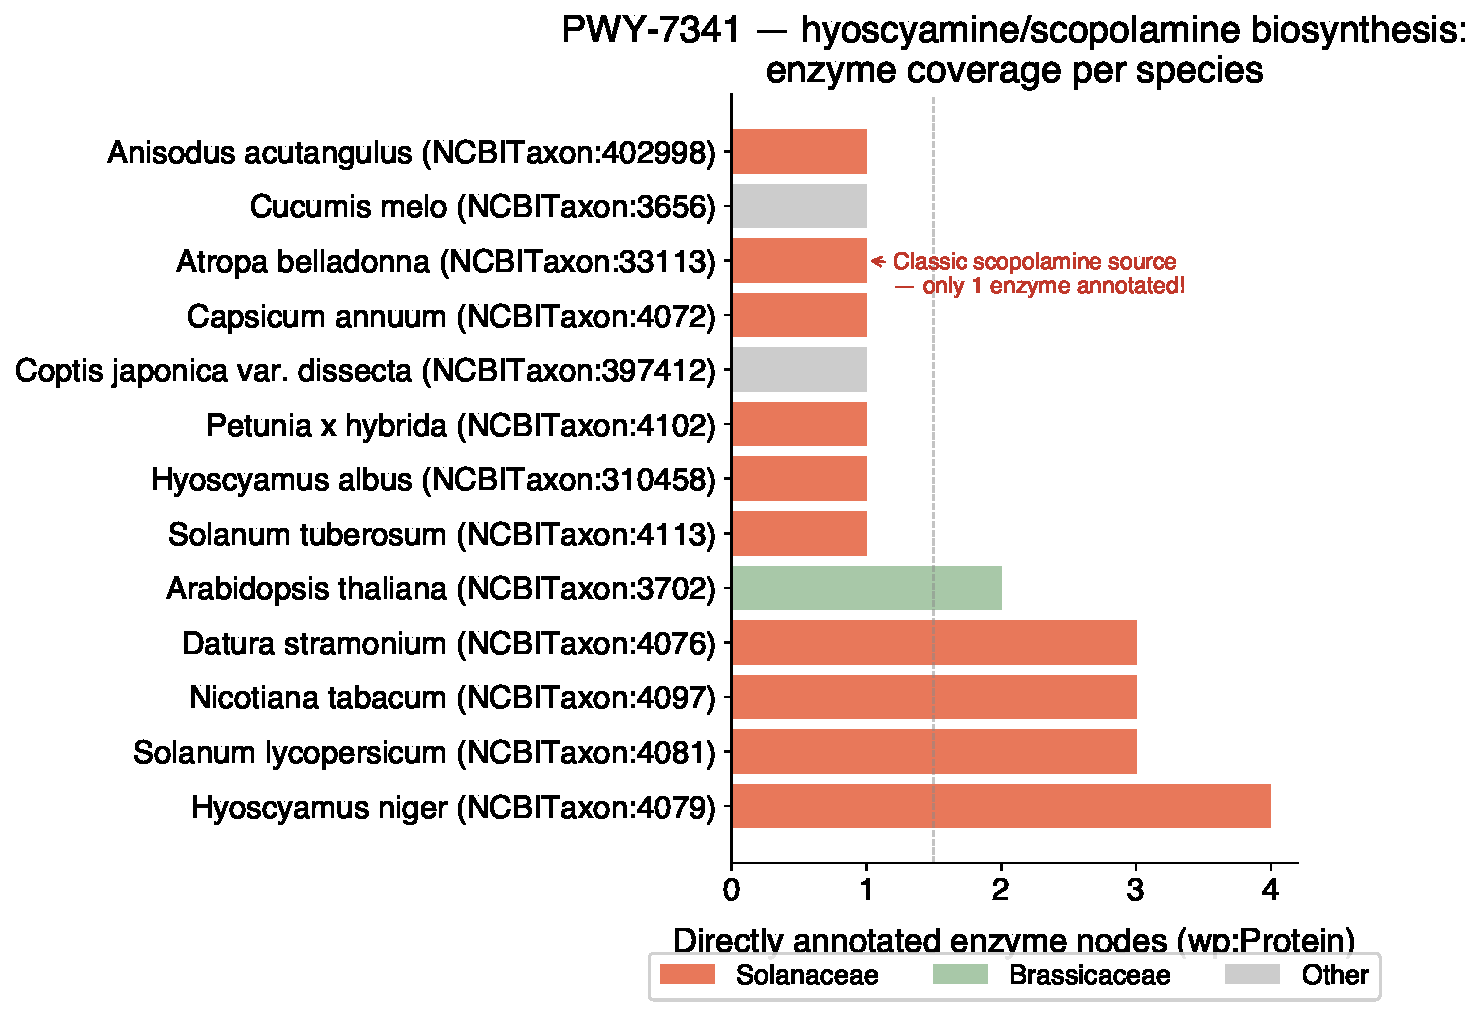
\includegraphics[width=0.78\textwidth]{supplementary_figures/figS13a.pdf}\\[1.0em]
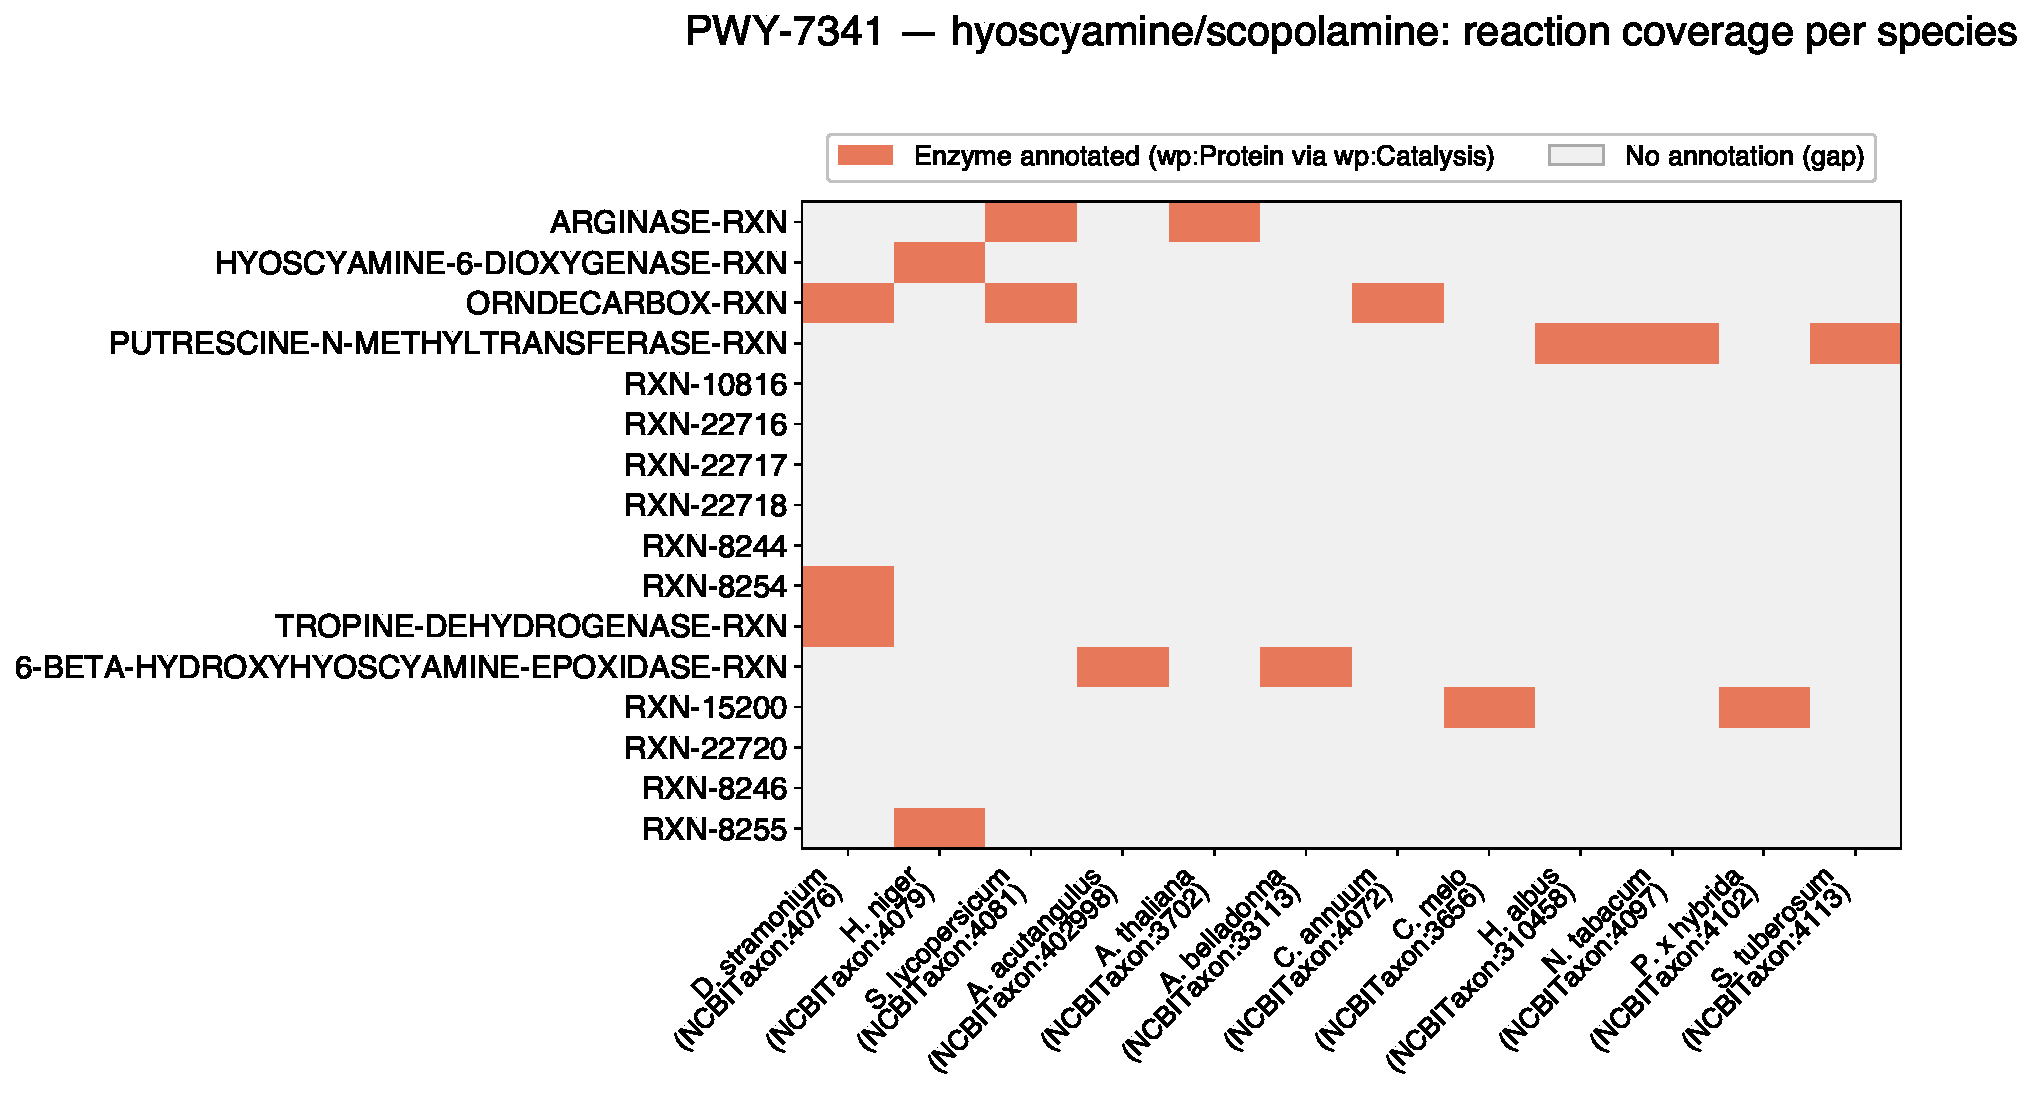
\includegraphics[width=0.88\textwidth]{supplementary_figures/figS13b.pdf}
\end{center}

\captionof{figure}{\footnotesize \textbf{Top panel: Enzyme coverage per species in
hyoscyamine/scopolamine biosynthesis (PWY-7341).} Bars show the count of directly annotated
\texttt{wp:Protein} enzyme nodes per species (NCBITaxon ID in parentheses). Orange = Solanaceae
species; green = Brassicaceae; grey = other families. \textit{Atropa belladonna}
(NCBITaxon:33113), the classical scopolamine source, has only 1 directly annotated enzyme despite
13 species being represented in this pathway, illustrating the curation asymmetry that
cross-species inference can address. \textit{Hyoscyamus niger} (NCBITaxon:4079) provides the most
complete annotation. \textbf{Bottom panel: Reaction coverage matrix for hyoscyamine/scopolamine
biosynthesis (PWY-7341).} Rows are \texttt{wp:Conversion} reactions (PlantCyc accession IDs);
columns are species with $\geq$1 annotated enzyme, labelled with abbreviated name and NCBITaxon
ID. Orange = reaction covered by an annotated \texttt{wp:Protein} via \texttt{wp:Catalysis};
grey = gap. Despite \textit{Atropa belladonna} being the principal pharmaceutical source of
scopolamine, its annotation depth is far below \textit{Hyoscyamus niger}, making it the primary
cross-species inference target in this pathway.}
\label{figS:scopolamine}

\clearpage

%------------------------------------------------------------------ S14
\begin{center}
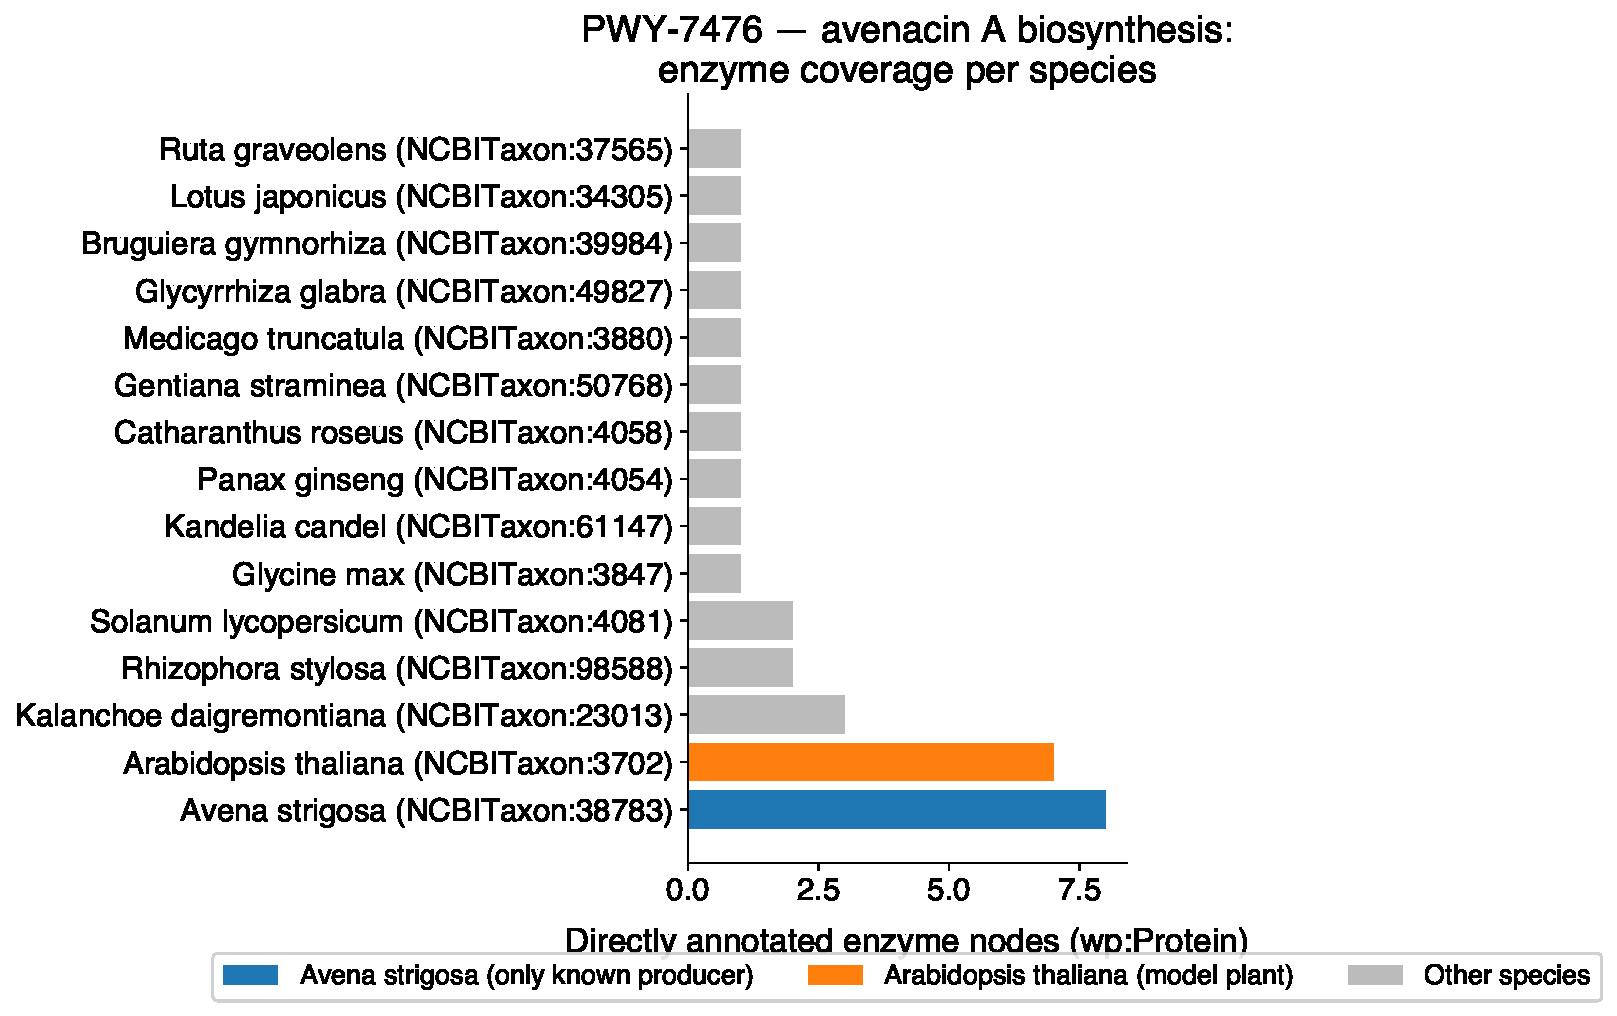
\includegraphics[width=0.90\textwidth]{supplementary_figures/figS14a.pdf}\\[1.0em]
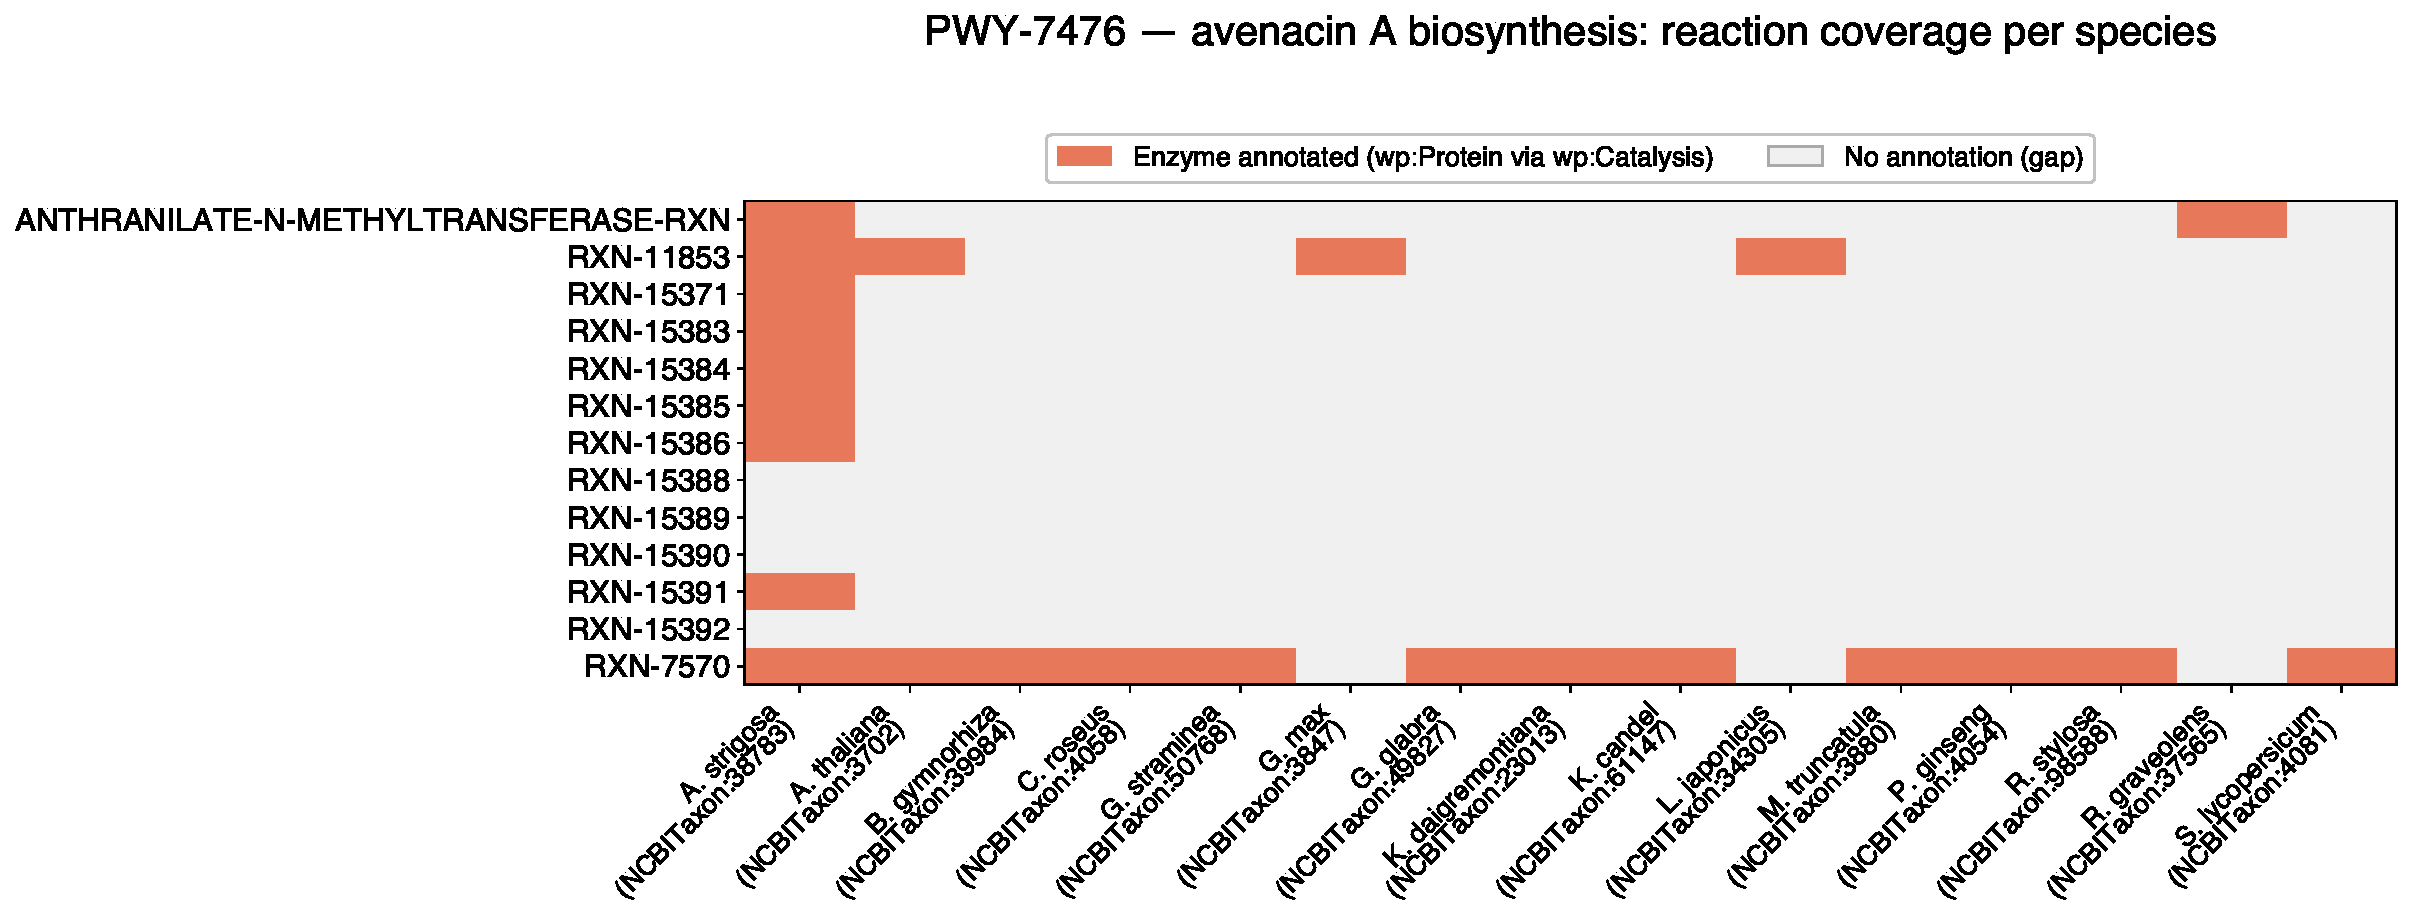
\includegraphics[width=\textwidth]{supplementary_figures/figS14b.pdf}
\end{center}

\captionof{figure}{\footnotesize \textbf{Top panel: Enzyme coverage per species in avenacin A biosynthesis
(PWY-7476).} Bars show directly annotated \texttt{wp:Protein} enzyme nodes per species (total
annotation depth). Blue = \textit{Avena strigosa} (NCBITaxon:38783, the only known producer);
orange = \textit{Arabidopsis thaliana} (NCBITaxon:3702, non-producer with orthologous triterpenoid
enzymes); grey = other species. Although \textit{Arabidopsis} carries nearly as many annotated
enzymes as \textit{Avena} at the enzyme level, at the reaction level it covers only 2 of 13
reactions, both of which are also covered in \textit{Avena} itself. \textbf{Bottom panel:
Reaction coverage matrix for avenacin A biosynthesis (PWY-7476).} Despite \textit{A. thaliana}
having comparable enzyme annotation depth to \textit{A. strigosa}, the reaction-level matrix
reveals a stark asymmetry: \textit{A. strigosa} covers 9 of 13 reactions while \textit{A.
thaliana} covers only 2, both shared with \textit{A. strigosa}. All \textit{A. thaliana}
annotation potential is therefore a cross-species transfer candidate, not independent evidence of
avenacin production in \textit{Arabidopsis}.}
\label{figS:avenacin}

\clearpage

%------------------------------------------------------------------ S15
\begin{center}
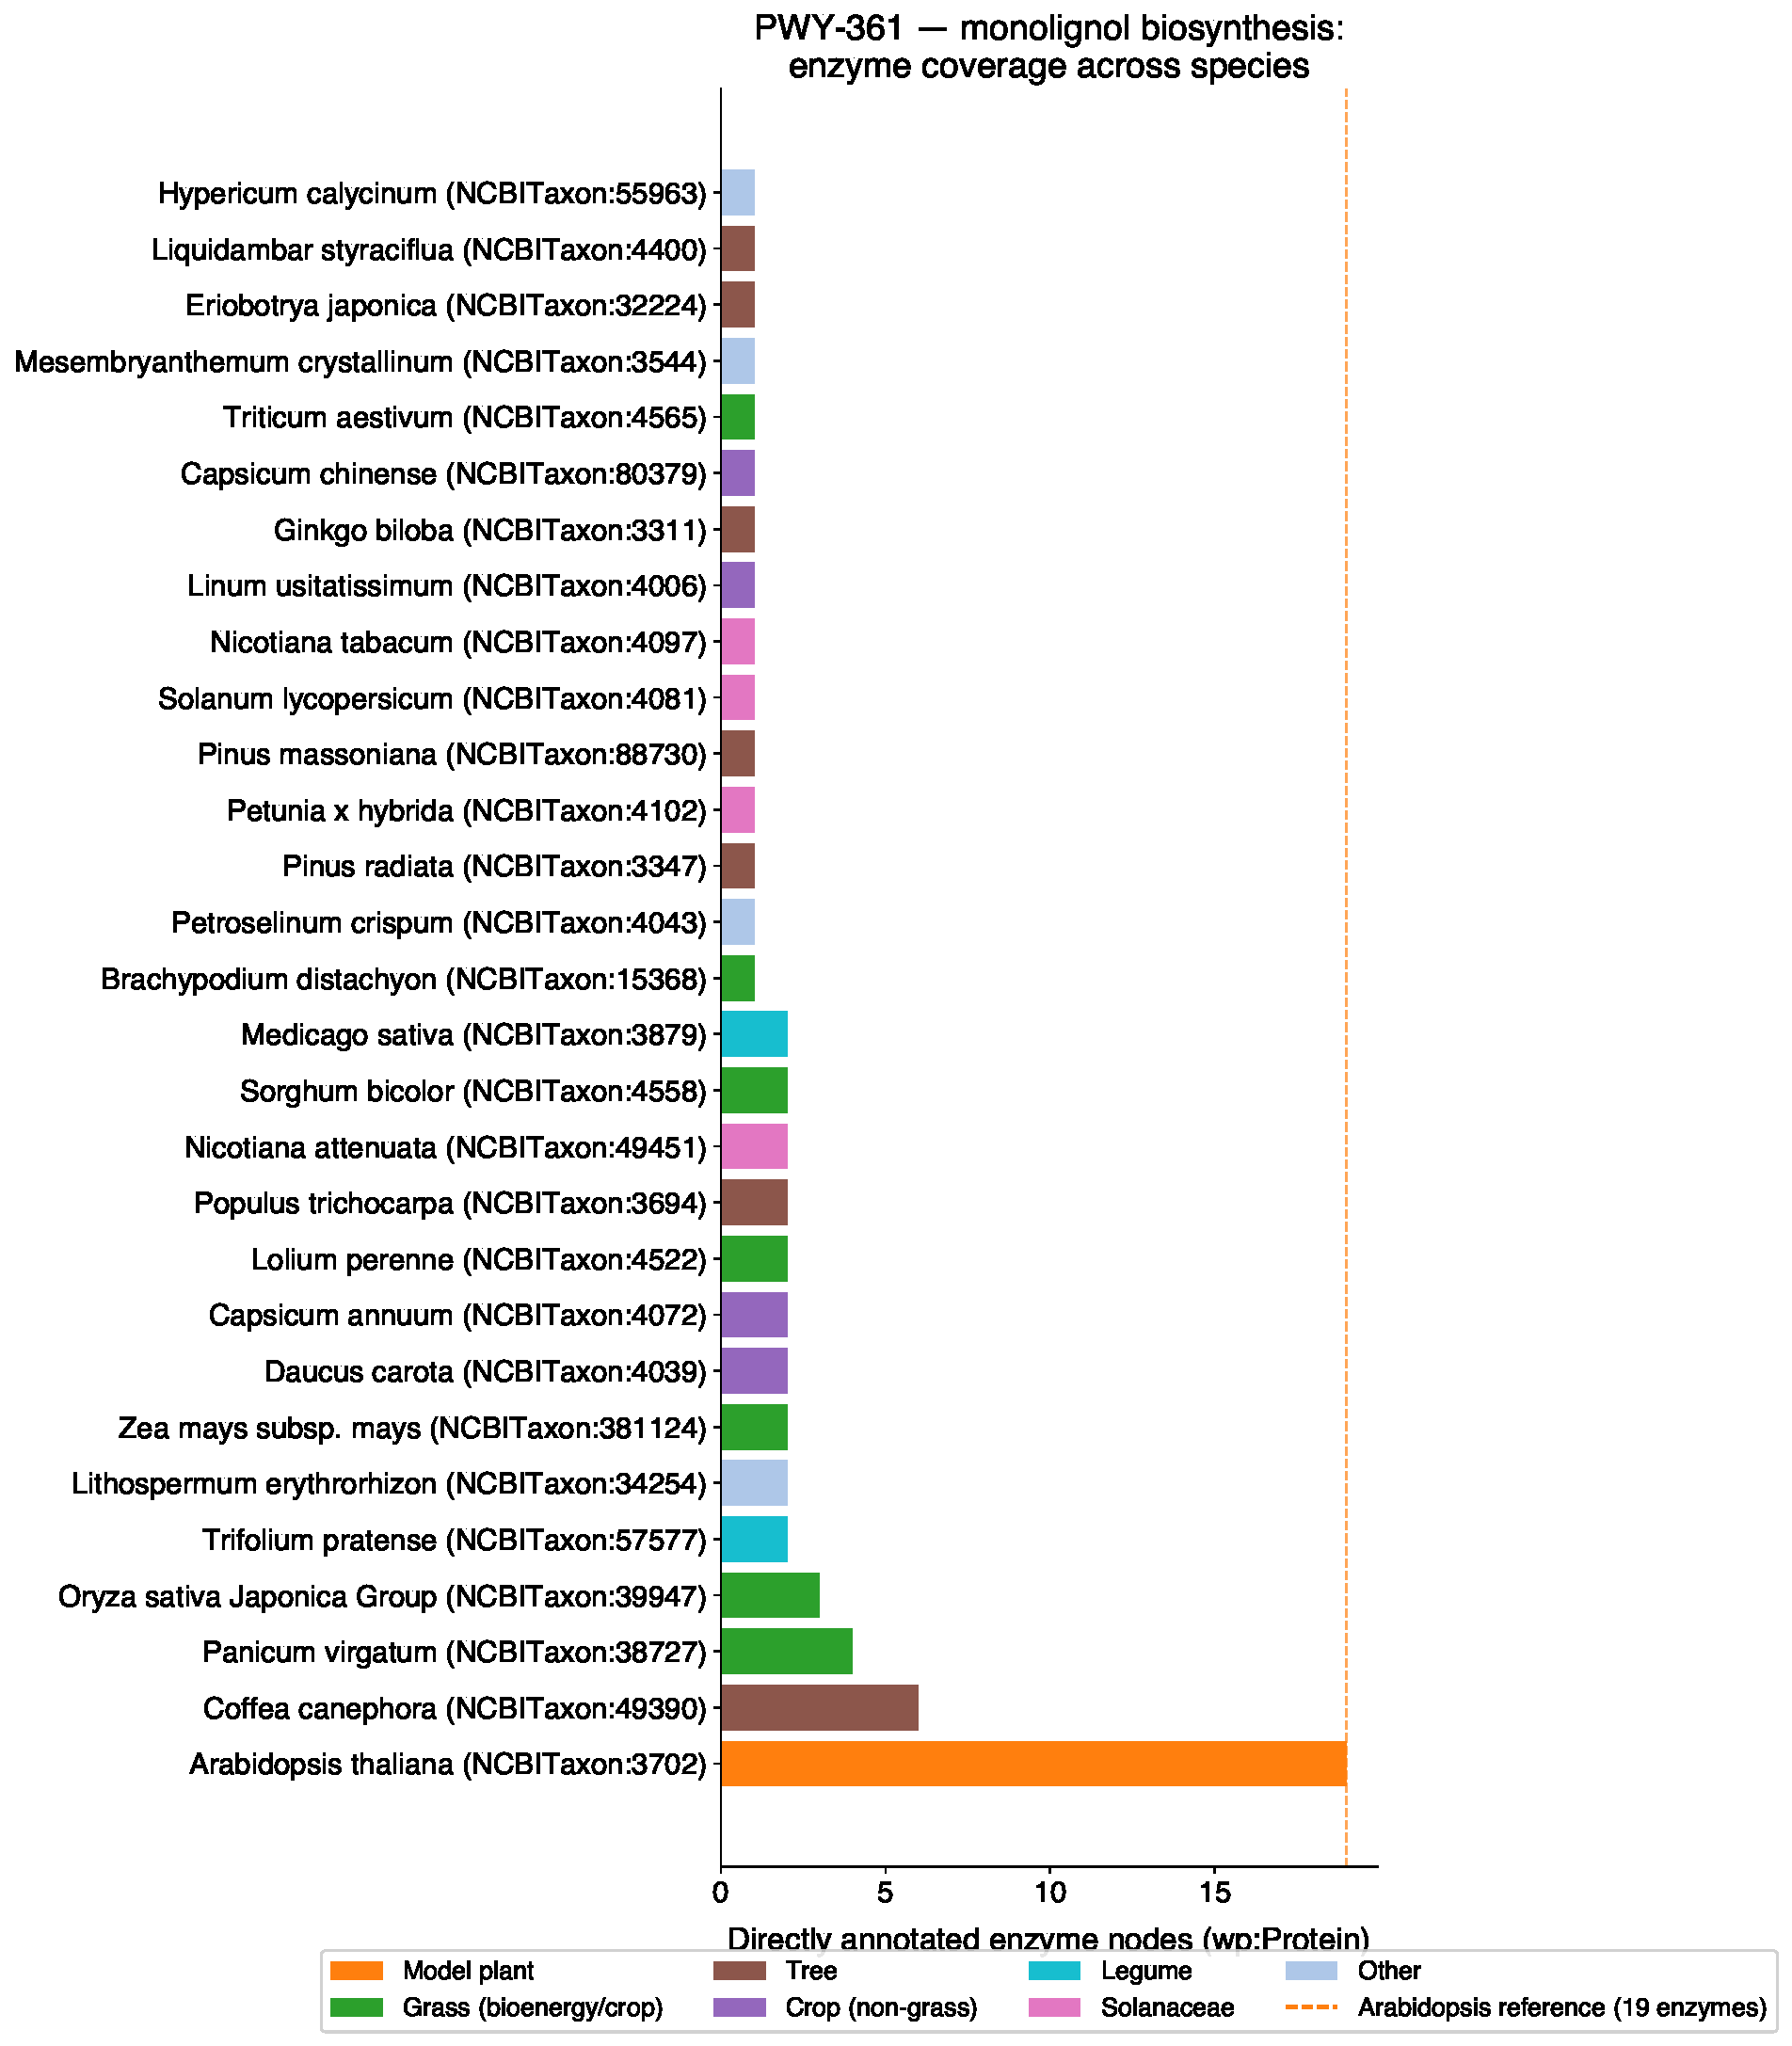
\includegraphics[height=0.40\textheight,keepaspectratio]{supplementary_figures/figS15a.pdf}\\[1.0em]
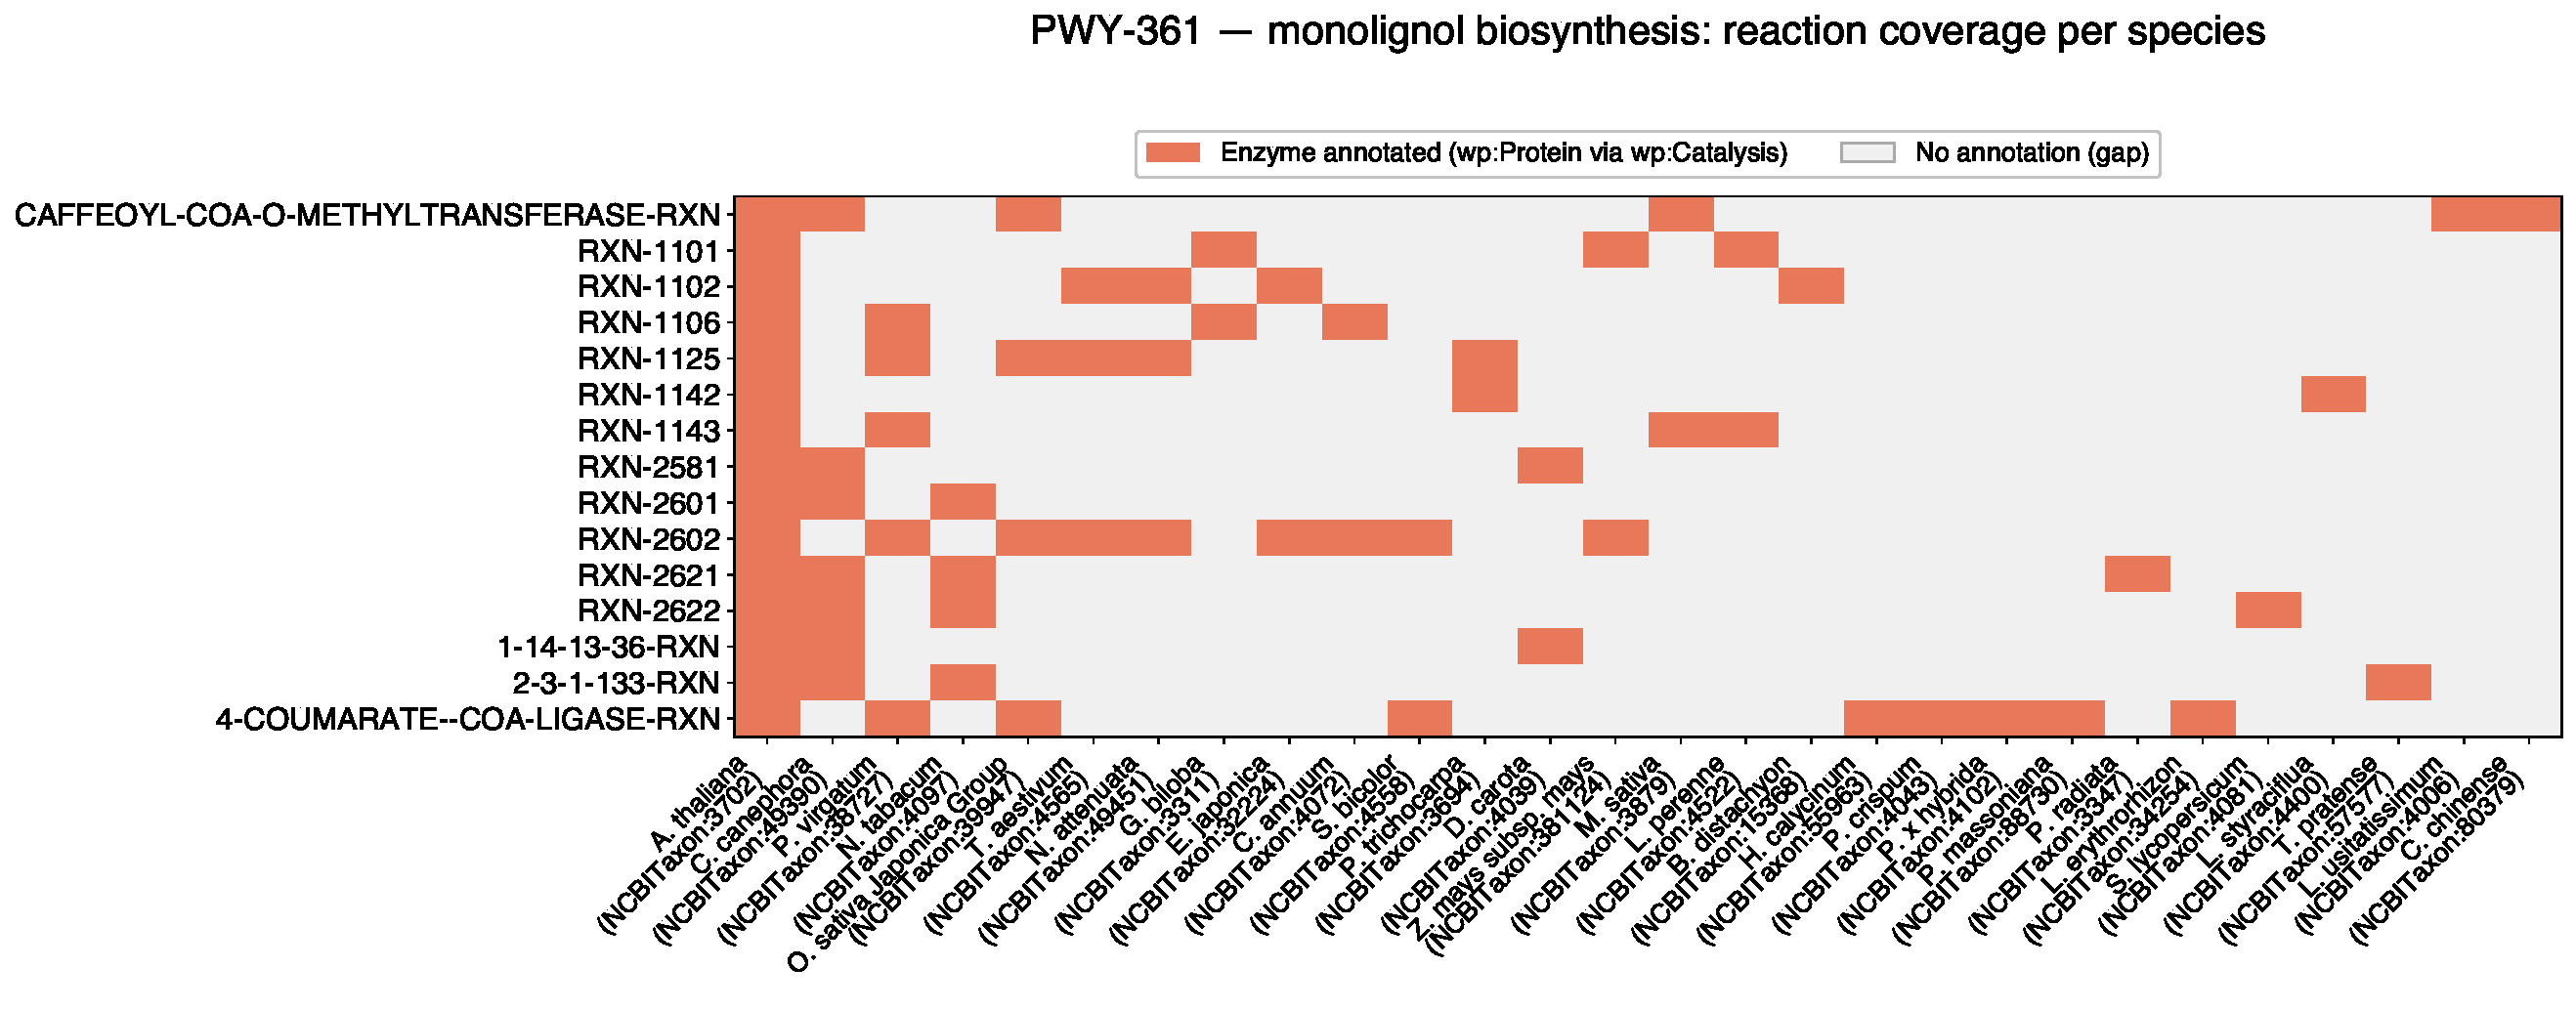
\includegraphics[width=0.95\textwidth]{supplementary_figures/figS15b.pdf}
\end{center}

\captionof{figure}{\footnotesize \textbf{Top panel: Enzyme coverage per species in monolignol biosynthesis
(PWY-361)}, the most taxonomically diverse pathway in PlantMetWiki (29 species). Species are
coloured by functional category (model plant, grass, tree, crop, legume, Solanaceae). The dashed
vertical line marks \textit{Arabidopsis thaliana}'s (NCBITaxon:3702) reference count of 19
annotated enzymes, the only species covering all 15 reactions in the pathway. Grasses (green bars)
show substantially lower coverage, motivating cross-species inference within the Poaceae family.
\textbf{Bottom panel: Reaction coverage matrix for monolignol biosynthesis (PWY-361).}
\textit{Arabidopsis thaliana} (NCBITaxon:3702) is the only species covering all 15 reactions; all
other species show substantial gaps. Within the Poaceae (grasses), the best-covered species reach
only 5 of 15 reactions, but combining annotations across the grass sub-family covers 13 of 15,
demonstrating the power of cross-family inference for biomass-relevant pathways.}
\label{figS:monolignol}

\clearpage

%------------------------------------------------------------------ S16
\begin{center}
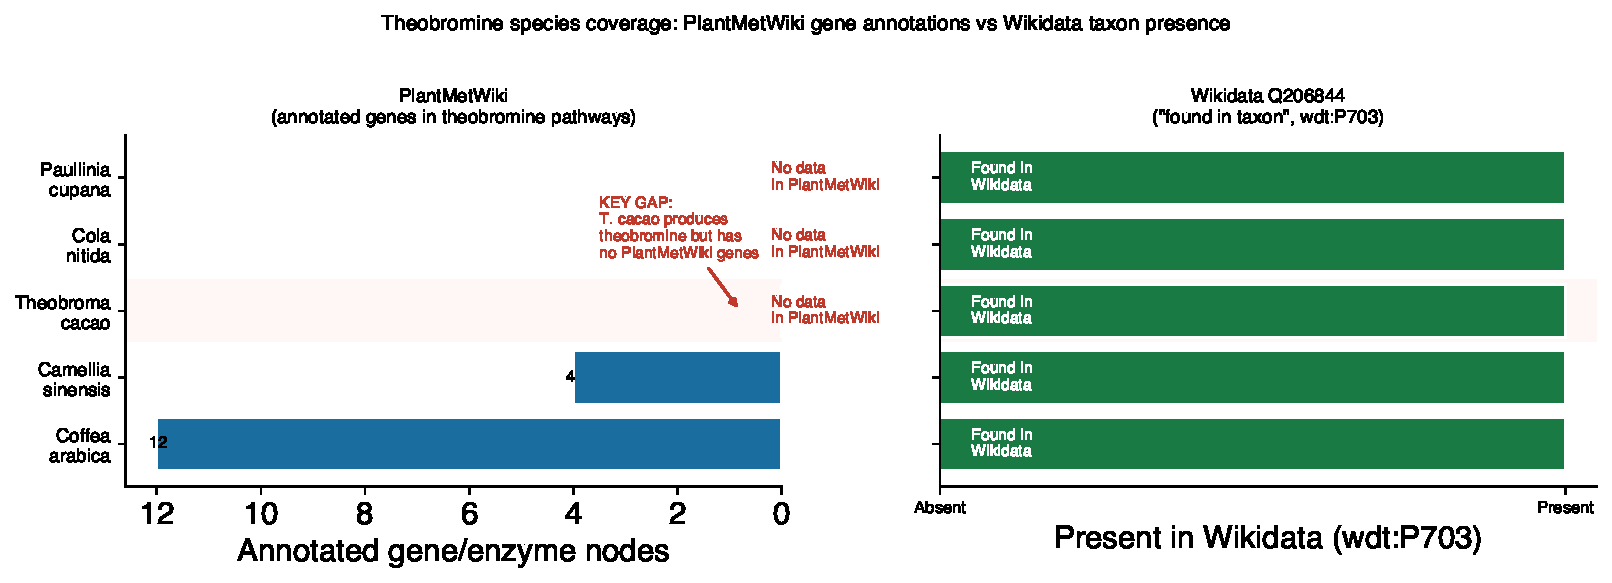
\includegraphics[width=\textwidth]{supplementary_figures/figS16.pdf}
\end{center}

\captionof{figure}{\footnotesize \textbf{Cross-species gap analysis for theobromine biosynthesis.} All
species known to produce theobromine according to Wikidata (\texttt{wdt:P703}, "found in taxon")
shown alongside their PlantMetWiki gene-annotation depth for theobromine-containing pathways.
How to read it: species present in Wikidata but with zero or low PlantMetWiki annotation
(\textit{Theobroma cacao}, \textit{Cola nitida} and \textit{Paullinia cupana}; only
\textit{Coffea arabica} and \textit{Camellia sinensis} are well annotated) are priority candidates
for annotation transfer, because Wikidata already provides taxonomic evidence that the pathway
should exist in these species.}
\label{figS:theobromine}

\clearpage

%------------------------------------------------------------------ S17
\begin{center}
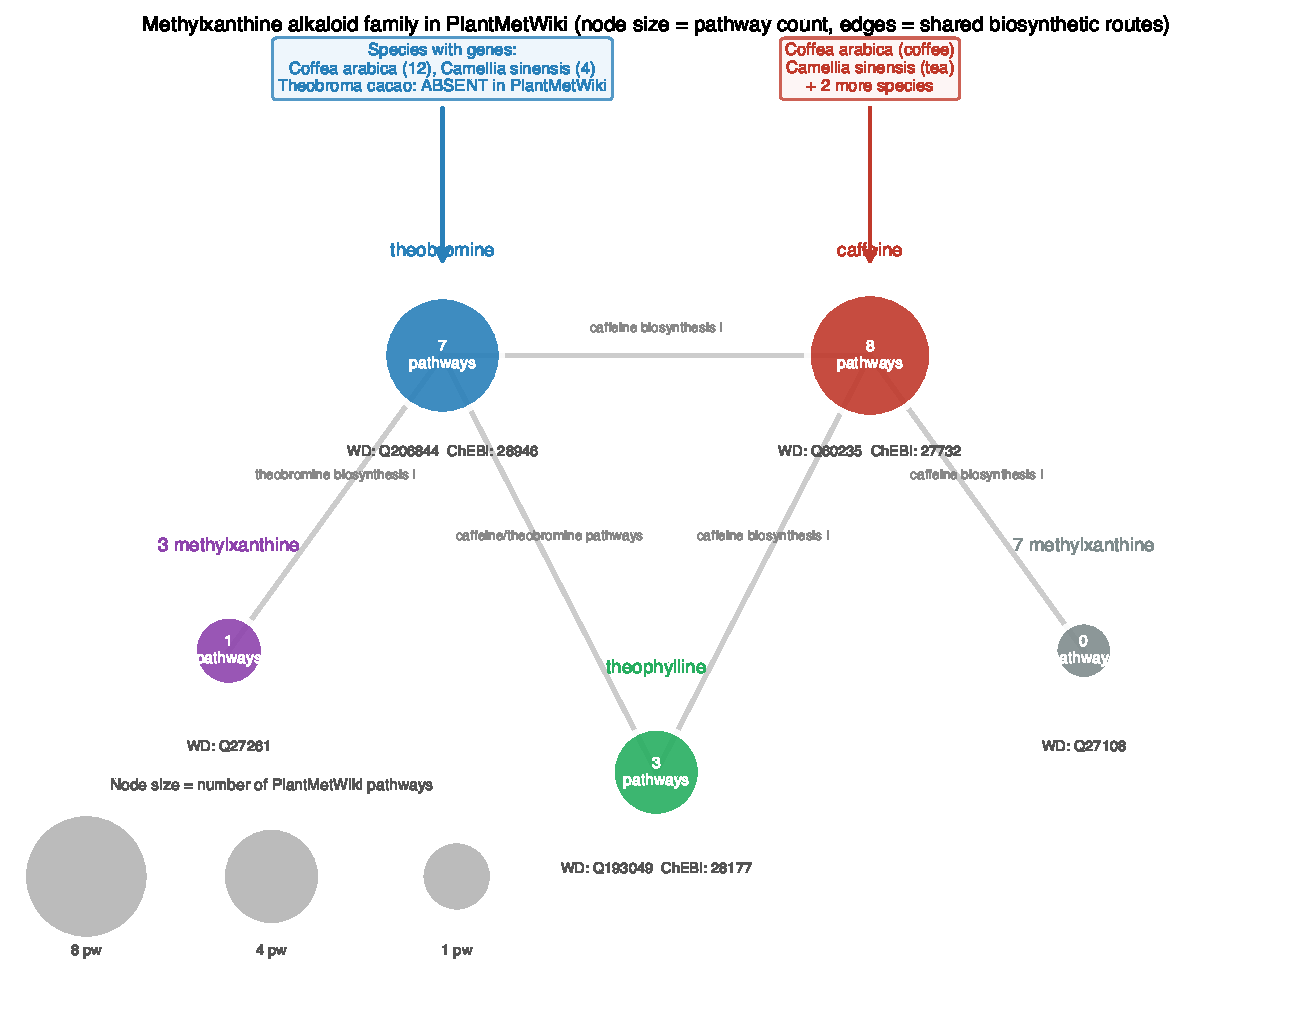
\includegraphics[width=0.95\textwidth]{supplementary_figures/figS17.pdf}
\end{center}

\captionof{figure}{\footnotesize \textbf{Methylxanthine metabolic family network.} Caffeine, theobromine,
theophylline and related methylxanthines, with node size proportional to the number of
PlantMetWiki pathways each compound appears in, and Wikidata QIDs / ChEBI IDs shown as
cross-reference labels. How to read it: larger, fully labelled nodes (caffeine: 8 pathways,
theobromine: 7) are well characterised in both PlantMetWiki and Wikidata; smaller nodes
(theophylline: 3 pathways, monomethylxanthines: 0) are progressively less curated.}
\label{figS:methylxanthine}

\clearpage

%------------------------------------------------------------------ S18
\begin{center}
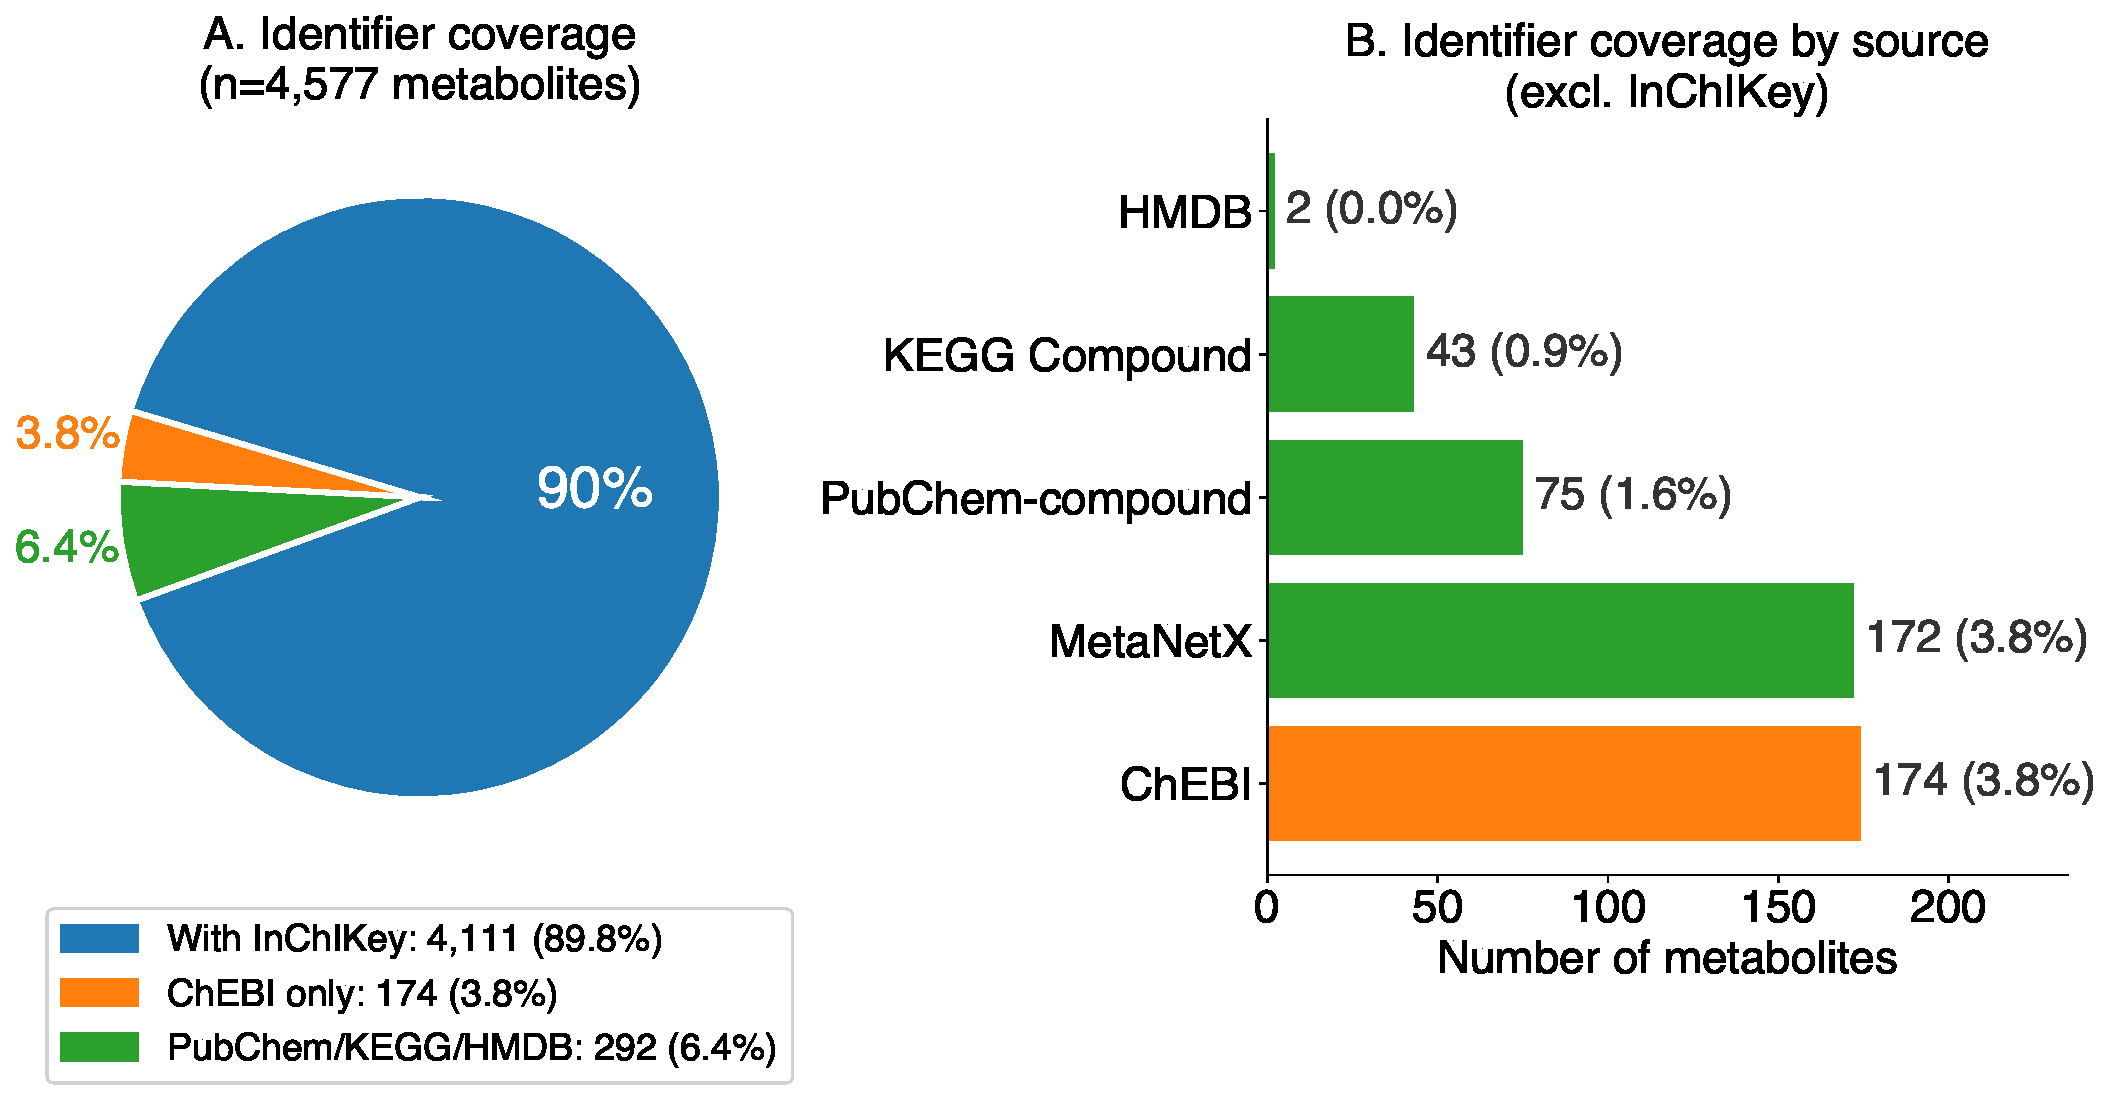
\includegraphics[width=\textwidth]{supplementary_figures/figS18.pdf}
\end{center}

\captionof{figure}{\footnotesize \textbf{Metabolite identifier coverage from PlantCyc (before BridgeDb
mapping).} \textbf{(A)} Identifier coverage across all 4,577 \texttt{wp:Metabolite} nodes in
PlantMetWiki: the proportion of metabolites carrying each external identifier type; 90\% (4,111)
have an InChIKey, the prerequisite for federated SPARQL queries to Wikidata via
\texttt{wdt:P235}. \textbf{(B)} Breakdown of the other cross-reference databases (ChEBI, MetaNetX,
PubChem, KEGG, HMDB) and how many metabolites carry each. As a result, 4,111 metabolites (90\%)
can be directly federated to Wikidata via InChIKey (\texttt{wdt:P235}).}
\label{figS:identifiercoverage}

\clearpage

%------------------------------------------------------------------ S19
\begin{center}
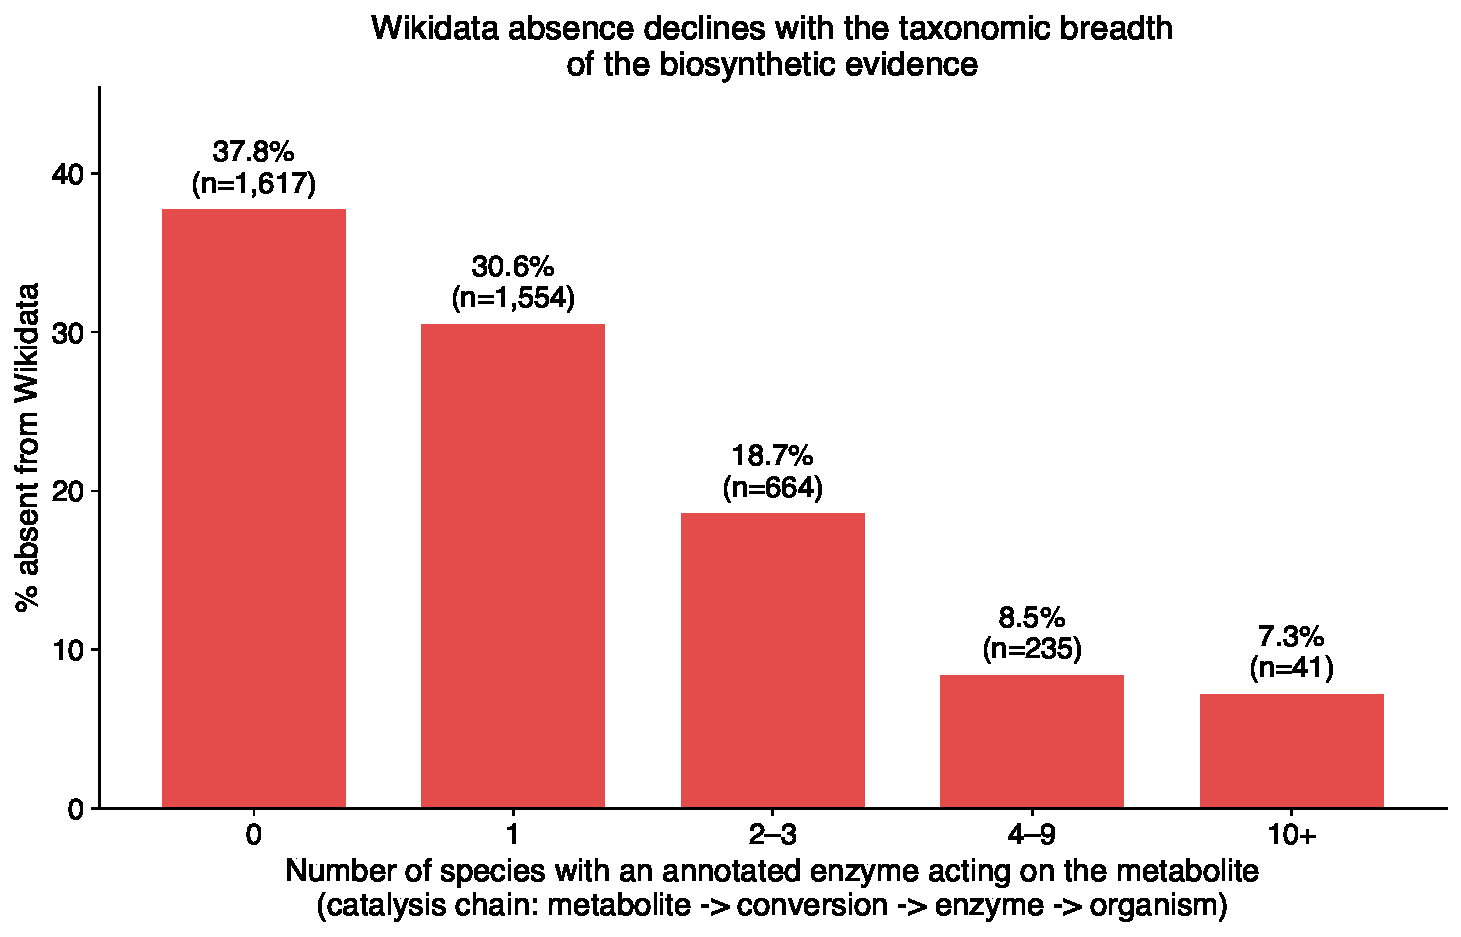
\includegraphics[width=0.95\textwidth]{supplementary_figures/figS19.pdf}
\end{center}

\captionof{figure}{\footnotesize \textbf{Wikidata absence declines with the taxonomic breadth of the
biosynthetic evidence.} For each of the 4,111 InChIKey-annotated PlantMetWiki metabolites,
taxonomic breadth is measured through the catalysis chain: the number of distinct species whose
annotated enzyme (\texttt{wp:Protein}, carrying \texttt{wp:organism}) catalyses a
\texttt{wp:Conversion} in which the metabolite participates (metabolite →
\texttt{wp:Conversion} → catalysing \texttt{wp:Protein} → \texttt{wp:organism}). Bars show the
percentage of metabolites in each breadth class that are absent from Wikidata by exact InChIKey;
bin sizes ($n$) are annotated. Absence falls steeply and monotonically, from 37.8\% for compounds
no annotated species produces ($n = 1{,}617$), to 30.6\% for a single species ($n = 1{,}554$),
18.7\% for two or three ($n = 664$), 8.5\% for four to nine ($n = 235$), and 7.3\% for ten or more
($n = 41$), showing that the Wikidata gap is concentrated in taxonomically restricted, specialized
plant chemistry.}
\label{figS:breadth}


\end{document}
